% Capitolul 5: Modele ARCH/GARCH pentru Volatilitate
% Prezentare academică de calitate Harvard
% Program de licență, Academia de Studii Economice din București

\documentclass[9pt, aspectratio=169, t]{beamer}

% Asigură încadrarea conținutului pe diapozitive
\setbeamersize{text margin left=8mm, text margin right=8mm}

%=============================================================================
% CONFIGURARE TEMĂ ȘI STIL
%=============================================================================
\usetheme{default}
% Tema implicită pentru control curat al antetului/subsolului

% Paletă de culori (conform PDF Redispatch)
\definecolor{MainBlue}{RGB}{26, 58, 110}
\definecolor{AccentBlue}{RGB}{26, 58, 110}
\definecolor{IDAred}{RGB}{205, 0, 0}
\definecolor{DarkGray}{RGB}{51, 51, 51}
\definecolor{MediumGray}{RGB}{128, 128, 128}
\definecolor{LightGray}{RGB}{248, 248, 248}
\definecolor{VeryLightGray}{RGB}{235, 235, 235}
\definecolor{KeynoteGray}{RGB}{218, 218, 218}
\definecolor{SectionGray}{RGB}{120, 120, 120}
\definecolor{FooterGray}{RGB}{100, 100, 100}
\definecolor{Crimson}{RGB}{220, 53, 69}
\definecolor{Forest}{RGB}{46, 125, 50}
\definecolor{Amber}{RGB}{181, 133, 63}
\definecolor{Orange}{RGB}{230, 126, 34}
\definecolor{Purple}{RGB}{142, 68, 173}

% Fundal gradient (gradient Keynote 315°: alb la RGB 218,218,218)
\setbeamertemplate{background}{%
    \begin{tikzpicture}[remember picture, overlay]
        \shade[shading=axis, shading angle=315,
        top color=white, bottom color=KeynoteGray]
        (current page.south west) rectangle (current page.north east);
    \end{tikzpicture}%
}
% Culoare solidă de rezervă pentru compatibilitate
\setbeamercolor{background canvas}{bg=}

\setbeamercolor{palette primary}{bg=MainBlue, fg=white}
\setbeamercolor{palette secondary}{bg=MainBlue!85, fg=white}
\setbeamercolor{palette tertiary}{bg=MainBlue!70, fg=white}
\setbeamercolor{structure}{fg=MainBlue}
\setbeamercolor{title}{fg=IDAred}
\setbeamercolor{frametitle}{fg=IDAred, bg=}
\setbeamercolor{block title}{bg=MainBlue, fg=white}
\setbeamercolor{block body}{bg=VeryLightGray, fg=DarkGray}
\setbeamercolor{block title alerted}{bg=Crimson, fg=white}
\setbeamercolor{block body alerted}{bg=Crimson!8, fg=DarkGray}
\setbeamercolor{block title example}{bg=Forest, fg=white}
\setbeamercolor{block body example}{bg=Forest!8, fg=DarkGray}
\setbeamercolor{item}{fg=MainBlue}

% Culori subsol (suprascrie albastrul temei Madrid)
\setbeamercolor{author in head/foot}{fg=FooterGray, bg=}
\setbeamercolor{title in head/foot}{fg=FooterGray, bg=}
\setbeamercolor{date in head/foot}{fg=FooterGray, bg=}
\setbeamercolor{section in head/foot}{fg=FooterGray, bg=}
\setbeamercolor{subsection in head/foot}{fg=FooterGray, bg=}

% Stiluri marcatori (aplicate inclusiv în blocuri)
\setbeamertemplate{itemize item}{\color{MainBlue}$\boxdot$}
\setbeamertemplate{itemize subitem}{\color{MainBlue}$\blacktriangleright$}
\setbeamertemplate{itemize subsubitem}{\color{MainBlue}\tiny$\bullet$}
\setbeamertemplate{itemize/enumerate body begin}{\normalsize}
\setbeamertemplate{itemize/enumerate subbody begin}{\normalsize}

% Item spacing - compact style
\setlength{\leftmargini}{10pt}       % Level 1: minimal indent
\setlength{\leftmarginii}{10pt}      % Level 2: minimal additional indent
% Compact list spacing (zero extra space before/after lists in blocks)
\makeatletter
\def\@listi{\leftmargin\leftmargini \topsep 0pt \parsep 0pt \itemsep 0pt}
\def\@listii{\leftmargin\leftmarginii \topsep 0pt \parsep 0pt \itemsep 0pt}
\makeatother

\setbeamertemplate{navigation symbols}{}

%=============================================================================
% CUSTOM HEADLINE
%=============================================================================
\setbeamertemplate{headline}{%
    \vskip10pt%
    \hbox to \paperwidth{%
        \hskip0.5cm%
        {\small\color{FooterGray}\renewcommand{\hyperlink}[2]{##2}\insertsectionhead}%
        \hfill%
        \textcolor{FooterGray}{\small\insertframenumber}%
        \hskip0.5cm%
    }%
    \vskip4pt%
    {\color{FooterGray}\hrule height 0.4pt}%
}

%=============================================================================
% CUSTOM FOOTER
%=============================================================================
\usepackage{fontawesome5}

\setbeamertemplate{footline}{%
    {\color{FooterGray}\hrule height 0.4pt}%
    \vskip4pt%
    \hbox to \paperwidth{%
        \hskip0.5cm%
        \textcolor{FooterGray}{\small Analiza și Prognoza Seriilor de Timp}%
        \hfill%
        \raisebox{-0.1em}{%
            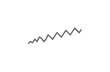
\begin{tikzpicture}[x=0.08em, y=0.08em, line width=0.4pt]
                \draw[FooterGray] (0,3) -- (1,4) -- (2,3.5) -- (3,5) -- (4,4) -- (5,6) -- (6,5.5) -- (7,4) -- (8,5) -- (9,7) -- (10,6) -- (11,5) -- (12,6.5) -- (13,8) -- (14,7) -- (15,6) -- (16,7.5) -- (17,9) -- (18,8) -- (19,7) -- (20,8.5) -- (21,10) -- (22,9) -- (23,8) -- (24,9.5);
            \end{tikzpicture}%
        }%
        \hskip0.5cm%
    }%
    \vskip6pt%
}

%=============================================================================
% PACHETE
%=============================================================================
\usepackage[utf8]{inputenc}
\usepackage[T1]{fontenc}
\usepackage{amsmath, amssymb, amsthm}
\usepackage{mathtools}
\usepackage{bm}
\usepackage{tikz}
\usetikzlibrary{arrows.meta, positioning, shapes, calc, decorations.pathreplacing, shadings}
\usepackage{booktabs}
\usepackage{multirow}
\usepackage{array}
\usepackage{graphicx}
\usepackage{hyperref}
\usepackage{colortbl}
\hypersetup{colorlinks=true, linkcolor=MainBlue, urlcolor=MainBlue}
\graphicspath{{../../logos/}{../../charts/}{../../photos/}}
\hfuzz=2pt  % Suppress tiny overfull warnings (<2pt)
\vfuzz=2pt  % Suppress tiny vertical overfull warnings (<2pt)

%=============================================================================
% COMANDA QUANTLET
%=============================================================================
\newcommand{\quantlet}[2]{%
    \hfill\href{#2}{%
        \raisebox{-0.15em}{\includegraphics[height=0.7em]{ql_logo.png}}%
        \textcolor{MainBlue}{\tiny\ #1}%
    }%
}

%=============================================================================
% MEDII PENTRU TEOREME
%=============================================================================
\theoremstyle{definition}
\setbeamertemplate{theorems}[numbered]
\newtheorem{defn}{Definiție}
\newtheorem{thm}{Teoremă}
\newtheorem{prop}{Propoziție}
\newtheorem{rmk}{Observație}

%=============================================================================
% CENTRED MINIPAGE (fără spațiu vertical suplimentar)
%=============================================================================
\newenvironment{cminipage}[1]{%
    \par\noindent\hfill\begin{minipage}{#1}\ignorespaces
}{%
    \end{minipage}\hfill\null\par
}

%=============================================================================
% COMENZI PERSONALIZATE
%=============================================================================
\newcommand{\E}{\mathbb{E}}
\newcommand{\Var}{\text{Var}}
\newcommand{\Cov}{\text{Cov}}
\newcommand{\Corr}{\text{Corr}}
\newcommand{\R}{\mathbb{R}}
\newcommand{\N}{\mathbb{N}}
\newcommand{\Z}{\mathbb{Z}}
\newcommand{\B}{\mathbf{B}}
\newcommand{\imark}{\textcolor{MainBlue}{\textbullet}}
\newcommand{\RMSE}{\text{RMSE}}
\newcommand{\MAE}{\text{MAE}}
\newcommand{\MAPE}{\text{MAPE}}

%=============================================================================
% PAGINĂ TITLU PERSONALIZATĂ
%=============================================================================
\defbeamertemplate*{title page}{hybrid}[1][]
{
    \vspace{0.2cm}
    % Logos row - top header (with clickable links)
    \begin{center}
        \href{https://www.ase.ro}{\includegraphics[height=1.0cm]{ase_logo.png}}\hspace{0.3cm}%
        \href{https://theida.net}{\includegraphics[height=1.0cm]{ida_logo.png}}\hspace{0.3cm}%
        \href{https://blockchain-research-center.com}{\includegraphics[height=1.0cm]{brc_logo.png}}\hspace{0.3cm}%
        \href{https://www.ai4efin.ase.ro}{\includegraphics[height=1.0cm]{ai4efin_logo.png}}\hspace{0.3cm}%
        \href{https://ipe.ro/new}{\includegraphics[height=1.0cm]{acad_logo.png}}\hspace{0.3cm}%
        \href{https://www.digital-finance-msca.com}{\includegraphics[height=1.0cm]{msca_logo.png}}%
    \end{center}

    \vspace{0.6cm}

    % Main title with Q logos on sides (with clickable links)
    \begin{center}
        \begin{minipage}{0.1\textwidth}
            \centering
            \href{https://quantlet.com}{\includegraphics[height=1.1cm]{ql_logo.png}}
        \end{minipage}%
        \begin{minipage}{0.78\textwidth}
            \centering
            {\LARGE\bfseries\usebeamercolor[fg]{title}\inserttitle}

            \vspace{0.3cm}

            {\usebeamerfont{subtitle}\usebeamercolor[fg]{title}\insertsubtitle}
        \end{minipage}%
        \begin{minipage}{0.1\textwidth}
            \centering
            \href{https://quantinar.com}{\includegraphics[height=1.1cm]{qr_logo.png}}
        \end{minipage}
    \end{center}

    \vspace{0.6cm}

    % Authors (left aligned)
    \hspace{0.5cm}{\usebeamerfont{author}\insertauthor}

    \vspace{0.3cm}

    % Institute/Affiliations (left aligned)
    \hspace{0.5cm}\begin{minipage}[t]{0.9\textwidth}
        \raggedright\small\insertinstitute
    \end{minipage}
}

%=============================================================================
% INFORMAȚII TITLU
%=============================================================================
\title[Analiza Seriilor de Timp]{Analiza și Prognoza Seriilor de Timp}
\subtitle{Capitolul 5: Modele ARCH/GARCH pentru Volatilitate}
\author[D.T. Pele]{Daniel Traian PELE}
\institute{Academia de Studii Economice din București\\
IDA Institute Digital Assets\\
Blockchain Research Center\\
AI4EFin Artificial Intelligence for Energy Finance\\
Academia Română, Institutul de Prognoză Economică\\
MSCA Digital Finance}
\date{}

\begin{document}

% Pagina de titlu (fără antet/subsol)
{
\setbeamertemplate{headline}{}
\setbeamertemplate{footline}{}
\begin{frame}
    \titlepage
\end{frame}
}

%=============================================================================
% OBIECTIVE DE ÎNVĂȚARE
%=============================================================================
\section{Motivație}

\begin{frame}{Obiective de învățare}
    \begin{cminipage}{0.95\textwidth}
    \begin{block}{La finalul acestui capitol, veți fi capabili să:}
        \begin{enumerate}\setlength{\itemsep}{0pt}
            \item Înțelegeți \textbf{volatility clustering} și faptele stilizate ale randamentelor financiare
            \item Estimați și interpretați modele \textbf{ARCH} și \textbf{GARCH}
            \item Aplicați modele asimetrice (\textbf{EGARCH}, \textbf{GJR-GARCH}) pentru efectul de levier
            \item Efectuați validarea și selectarea modelelor
            \item Prognozați volatilitatea și calculați \textbf{Value at Risk (VaR)}
        \end{enumerate}
    \end{block}
    \vspace{-0.1cm}
    \begin{alertblock}{Competențe practice}
        \begin{itemize}\setlength{\itemsep}{0pt}
            \item Implementare Python cu pachetul \texttt{arch}
                \begin{itemize}\setlength{\itemsep}{0pt}
                    \item Estimare, prognoză și diagnostic automat
                \end{itemize}
            \item Interpretarea parametrilor și a persistenței volatilității
            \item Calculul VaR pentru managementul riscului
                \begin{itemize}\setlength{\itemsep}{0pt}
                    \item Backtesting și validarea prognozelor
                \end{itemize}
        \end{itemize}
    \end{alertblock}
    \end{cminipage}
\end{frame}

%=============================================================================
% CUPRINS
%=============================================================================
\begin{frame}{Cuprins}
    \vspace{-0.3cm}
    {\small
    \begin{columns}[T]
        \begin{column}{0.48\textwidth}
            \begin{block}{Fundamente}
                \begin{itemize}\setlength{\itemsep}{3pt}
                    \item Motivație
                    \item Introducere în Modelarea Volatilității
                    \item Modelul ARCH
                    \item Modelul GARCH
                    \item Modele GARCH Asimetrice
                    \item Selectarea și Diagnosticarea modelelor
                \end{itemize}
            \end{block}
        \end{column}
        \begin{column}{0.48\textwidth}
            \begin{exampleblock}{Aplicații}
                \begin{itemize}\setlength{\itemsep}{3pt}
                    \item Prognoza volatilității
                    \item Implementare în Python
                    \item Studiu de Caz: S\&P 500
                    \item Studiu de Caz: Bitcoin
                    \item Rezumat și Quiz
                \end{itemize}
            \end{exampleblock}
        \end{column}
    \end{columns}
    }
\end{frame}

%=============================================================================
% SECȚIUNEA 1: INTRODUCERE ÎN MODELAREA VOLATILITĂȚII
%=============================================================================
\section{Introducere în Modelarea Volatilității}

\begin{frame}{Volatility clustering}
    \vspace{-0.2cm}
    {\footnotesize
    \begin{block}{Observații}
            \begin{itemize}\setlength{\itemsep}{0pt}
                \item Perioadele de volatilitate mare sunt urmate de perioade similare
                \item Perioadele de calm sunt urmate de perioade de calm
                \item Varianța condiționată este \textbf{predictibilă}
            \end{itemize}
        \end{block}
    }
    \begin{center}
        \includegraphics[width=0.95\textwidth, height=0.50\textheight, keepaspectratio]{garch_volatility_clustering.pdf}
    \end{center}
    \quantlet{TSA\_ch5\_clustering}{https://github.com/QuantLet/TSA/tree/main/TSA_ch5/TSA_ch5_clustering}
\end{frame}

\begin{frame}{De ce modelăm volatilitatea?}
\small
    \begin{cminipage}{0.95\textwidth}
    \begin{block}{Observații empirice în seriile financiare}
        \begin{itemize}\setlength{\itemsep}{0pt}
            \item Randamentele prezintă \textbf{volatility clustering}
                \begin{itemize}\setlength{\itemsep}{0pt}
                    \item Perioadele de volatilitate ridicată sunt urmate de perioade similare
                \end{itemize}
            \item Distribuția randamentelor are \textbf{cozi groase} (leptokurtosis)
                \begin{itemize}\setlength{\itemsep}{0pt}
                    \item Kurtosis $> 3$, mai multe valori extreme decât normala
                \end{itemize}
            \item Corelația randamentelor $\approx 0$, dar corelația $r_t^2$ este semnificativă
            \item Volatilitatea răspunde \textbf{asimetric} la șocuri (leverage effect)
        \end{itemize}
    \end{block}

    \vspace{0.2cm}

    \begin{alertblock}{Limitarea modelelor ARIMA}
        \begin{itemize}\setlength{\itemsep}{0pt}
            \item Modelele ARIMA presupun \textbf{varianță constantă} (homoscedasticitate)
                \begin{itemize}\setlength{\itemsep}{0pt}
                    \item Nu pot modela schimbările dinamice ale volatilității
                \end{itemize}
            \item Soluția: modele ARCH/GARCH pentru varianța condiționată
        \end{itemize}
    \end{alertblock}
    \end{cminipage}
\end{frame}

\begin{frame}{Exemplu: Bitcoin $\succ$ volatility clustering}
    \vspace{-0.2cm}
    \begin{center}
        \includegraphics[width=0.95\textwidth, height=0.46\textheight, keepaspectratio]{btc_returns.pdf}
    \end{center}
    \vspace{-0.2cm}
    {\footnotesize
    \begin{block}{Observații}
        \begin{itemize}\setlength{\itemsep}{0pt}
            \item Randamente zilnice Bitcoin (2019--2025): volatility clustering extrem de pronunțat
                \begin{itemize}\setlength{\itemsep}{0pt}
                    \item Randamente de $\pm 20\%$ în perioadele de criză (COVID, Terra/Luna)
                \end{itemize}
            \item Volatilitatea Bitcoin este semnificativ mai mare decât a activelor tradiționale
                \begin{itemize}\setlength{\itemsep}{0pt}
                    \item $\alpha$ tipic $\approx 0.10$--$0.20$ (reacție rapidă la news)
                \end{itemize}
        \end{itemize}
    \end{block}
    }
    \quantlet{TSA\_ch5\_btc\_returns}{https://github.com/QuantLet/TSA/tree/main/TSA_ch5/TSA_ch5_btc_returns}
\end{frame}

\begin{frame}{Fapte stilizate ale randamentelor financiare}
    \vspace{-0.2cm}
    {\scriptsize
    \begin{block}{Proprietăți observate}
        \begin{itemize}\setlength{\itemsep}{0pt}
            \item \textbf{Absența autocorelației} în randamente, dar \textbf{autocorelație semnificativă} în $r_t^2$
            \item \textbf{Cozi groase} (kurtosis $> 3$), \textbf{leverage effect}, \textbf{volatility clustering}
        \end{itemize}
    \end{block}
    }
    \begin{center}
        \includegraphics[width=0.95\textwidth, height=0.50\textheight, keepaspectratio]{garch_stylized_facts.pdf}
    \end{center}
    \quantlet{TSA\_ch5\_stylized}{https://github.com/QuantLet/TSA/tree/main/TSA_ch5/TSA_ch5_stylized}
\end{frame}

\begin{frame}{Exemplu: Bitcoin $\succ$ evidență pentru efecte ARCH}
    \vspace{-0.2cm}
    {\scriptsize
    \begin{cminipage}{0.95\textwidth}
    \vspace{-0.3cm}
    \vspace{-0.2cm}
    {\footnotesize
    \begin{block}{Interpretare}
        \begin{itemize}\setlength{\itemsep}{0pt}
            \item \textbf{Sus}: $r_t^2$ (proxy pentru volatilitate) $\succ$ vârfurile coincid cu crizele de piață
            \item \textbf{Jos}: ACF($r_t^2$) semnificativ $\succ$ efecte ARCH prezente, varianță predictibilă
        \end{itemize}
    \end{block}
    }
    \end{cminipage}
    }
    \begin{center}
        \includegraphics[width=0.95\textwidth, height=0.50\textheight, keepaspectratio]{btc_acf_squared.pdf}
    \end{center}
    \quantlet{TSA\_ch5\_btc\_arch}{https://github.com/QuantLet/TSA/tree/main/TSA_ch5/TSA_ch5_btc_arch}
\end{frame}

\begin{frame}{Heteroscedasticitate condiționată}
\small
    \begin{cminipage}{0.95\textwidth}
    \begin{defn}[Varianță Condiționată]
        \begin{itemize}\setlength{\itemsep}{0pt}
            \item \textbf{Definiție}: Fie $\{r_t\}$ o serie de randamente. Varianța condiționată la momentul $t$ este:
            \[
                \sigma_t^2 = \Var(r_t | \mathcal{F}_{t-1}) = \E[(r_t - \mu_t)^2 | \mathcal{F}_{t-1}]
            \]
            \item \textbf{Notație}: $\mathcal{F}_{t-1}$ reprezintă informația disponibilă până la momentul $t-1$
        \end{itemize}
    \end{defn}

    \vspace{0.2cm}

    \begin{block}{Modelul general}
        \begin{itemize}\setlength{\itemsep}{0pt}
            \item \textbf{Ecuația}: $r_t = \mu_t + \varepsilon_t$, \; $\varepsilon_t = \sigma_t z_t$, \; $z_t \sim \text{i.i.d.}(0, 1)$
            \item $\mu_t$ = media condiționată (modelată prin ARMA)
            \item $\sigma_t^2$ = varianța condiționată (modelată prin GARCH)
            \item $z_t$ = inovații standardizate
        \end{itemize}
    \end{block}
    \end{cminipage}
\end{frame}

%=============================================================================
% SECȚIUNEA 2: MODELUL ARCH
%=============================================================================
\section{Modelul ARCH}

\begin{frame}{Portret de cercetător: Engle \& Bollerslev}
    \vspace{-0.2cm}
    \begin{columns}[T]
        \begin{column}{0.22\textwidth}
            \centering
            \includegraphics[width=0.95\textwidth, height=0.22\textheight, keepaspectratio]{photo_robert_engle.jpg}
            \\[0.05cm]
            {\tiny\textcolor{MediumGray}{Robert Engle (*1942)}}\\[-0.05cm]
            {\tiny\textcolor{MediumGray}{Premiul Nobel 2003}}\\[0.02cm]
            \href{https://en.wikipedia.org/wiki/Robert_F._Engle}{\faWikipediaW\ \textcolor{MainBlue}{\tiny Wikipedia (en)}}
        \end{column}
        \begin{column}{0.76\textwidth}
            \begin{block}{Biografie}
                {\footnotesize \begin{itemize}\setlength{\itemsep}{0pt}
                    \item \textbf{Robert Engle}: economist american la NYU Stern. Premiul Nobel (2003) ,,pentru metode de analiză a seriilor economice cu volatilitate variabilă în timp (ARCH)''
                    \item \textbf{Tim Bollerslev}: economist danez-american la Duke University, doctorand al lui Engle
                \end{itemize}}
            \end{block}
        \end{column}
    \end{columns}
    \vspace{0.1cm}
    \begin{columns}[T]
        \begin{column}{0.22\textwidth}
            \centering
            \includegraphics[width=0.95\textwidth, height=0.22\textheight, keepaspectratio]{photo_tim_bollerslev.jpg}
            \\[0.05cm]
            {\tiny\textcolor{MediumGray}{Tim Bollerslev (*1958)}}\\[0.02cm]
            \href{https://en.wikipedia.org/wiki/Tim_Bollerslev}{\faWikipediaW\ \textcolor{MainBlue}{\tiny Wikipedia (en)}}
        \end{column}
        \begin{column}{0.76\textwidth}
            \begin{exampleblock}{Contribuții principale}
                {\footnotesize
                \begin{itemize}\setlength{\itemsep}{0pt}
                    \item \textbf{Modelul ARCH} (Engle, 1982) --- heteroskedasticitate condiționată autoregresivă
                    \item \textbf{Modelul GARCH} (Bollerslev, 1986) --- ARCH generalizat cu volatilitate persistentă
                    \item \textbf{Volatilitatea realizată} și econometria de înaltă frecvență
                    \item Fundamentul managementului modern al riscului financiar (VaR, ES)
                \end{itemize}}
            \end{exampleblock}
        \end{column}
    \end{columns}
\end{frame}

\begin{frame}{Simulare ARCH(1): Efectul parametrului $\alpha$}
    \vspace{-0.2cm}
    {\scriptsize
    \begin{block}{Interpretare}
        \begin{itemize}\setlength{\itemsep}{0pt}
            \item Cu cât $\alpha$ este mai mare, cu atât volatilitatea reacționează mai puternic la șocuri recente
        \end{itemize}
    \end{block}
    }
    \begin{center}
        \includegraphics[width=0.95\textwidth, height=0.50\textheight, keepaspectratio]{garch_arch1_simulation.pdf}
    \end{center}
    \quantlet{TSA\_ch5\_arch\_sim}{https://github.com/QuantLet/TSA/tree/main/TSA_ch5/TSA_ch5_arch_sim}
\end{frame}

\begin{frame}{Modelul ARCH(q) $\succ$ Engle (1982)}
    \vspace{-0.2cm}
\small
    \begin{cminipage}{0.95\textwidth}
    \begin{defn}[ARCH(q)]
        \begin{itemize}\setlength{\itemsep}{0pt}
            \item \textbf{Model}: Autoregressive Conditional Heteroskedasticity de ordin $q$:
            \vspace{-0.2cm}
            \[
                \varepsilon_t = \sigma_t z_t, \quad z_t \sim \text{i.i.d.}(0, 1), \quad
                \sigma_t^2 = \omega + \sum_{i=1}^{q} \alpha_i \varepsilon_{t-i}^2
            \]
        \end{itemize}
    \end{defn}
    \vspace{-0.2cm}
    \begin{block}{Restricții pentru staționaritate}
        \begin{itemize}\setlength{\itemsep}{0pt}
            \item $\omega > 0$ $\succ$ nivel de bază pozitiv
            \item $\alpha_i \geq 0$ pentru $i = 1, \ldots, q$ $\succ$ non-negativitate
            \item $\sum_{i=1}^{q} \alpha_i < 1$ $\succ$ staționaritate (varianță necondiționată finită)
        \end{itemize}
    \end{block}
    \vspace{-0.1cm}
    \begin{rmk}
        \begin{itemize}\setlength{\itemsep}{0pt}
            \item Robert Engle a primit \textbf{Premiul Nobel pentru Economie} în 2003 pentru dezvoltarea modelului ARCH!
        \end{itemize}
    \end{rmk}
    \end{cminipage}
\end{frame}

\begin{frame}{Proprietăți ale modelului ARCH(1)}
    \begin{cminipage}{0.95\textwidth}
    \begin{block}{ARCH(1): $\sigma_t^2 = \omega + \alpha_1 \varepsilon_{t-1}^2$}
        \begin{itemize}\setlength{\itemsep}{0pt}
            \item \textbf{Varianța necondiționată}: $\E[\varepsilon_t^2] = \dfrac{\omega}{1 - \alpha_1}$ (dacă $\alpha_1 < 1$)
            \item \textbf{Kurtosis}: $\kappa = 3 \cdot \dfrac{1 - \alpha_1^2}{1 - 3\alpha_1^2}$ (dacă $\alpha_1^2 < 1/3$)
            \item Kurtosis $> 3$ pentru $\alpha_1 > 0$ $\succ$ \textbf{cozi groase}!
        \end{itemize}
    \end{block}

    \vspace{0.3cm}

    \begin{exampleblock}{Exemplu numeric: $\omega = 0.0001$, $\alpha_1 = 0.3$}
        \begin{itemize}\setlength{\itemsep}{0pt}
            \item \textbf{Varianța necondiționată}: $\sigma^2 = \frac{0.0001}{1 - 0.3} = 0.000143$
            \item \textbf{Kurtosis}: $\kappa = 3 \cdot \frac{1 - 0.09}{1 - 0.27} = 3.74 > 3$
        \end{itemize}
    \end{exampleblock}
    \end{cminipage}
\end{frame}

%=============================================================================
% DEMONSTRAȚII
%=============================================================================

\begin{frame}{Demonstrație: varianța necondiționată ARCH(1)}
    \begin{cminipage}{0.95\textwidth}
    \begin{block}{Obiectiv}
        \begin{itemize}\setlength{\itemsep}{0pt}
            \item \textbf{Scop}: pentru ARCH(1): $\sigma_t^2 = \omega + \alpha\varepsilon_{t-1}^2$, demonstrăm $\E[\varepsilon_t^2] = \frac{\omega}{1-\alpha}$
        \end{itemize}
    \end{block}
    \vspace{-0.1cm}
    \begin{block}{Demonstrație}
        \begin{itemize}\setlength{\itemsep}{0pt}
            \item \textbf{Pas 1}: Legea speranțelor iterate: $\E[\varepsilon_t^2] = \E[\E[\varepsilon_t^2 | \mathcal{F}_{t-1}]] = \E[\sigma_t^2]$
            \item \textbf{Pas 2}: Înlocuim ARCH(1): $\E[\sigma_t^2] = \E[\omega + \alpha\varepsilon_{t-1}^2] = \omega + \alpha\E[\varepsilon_{t-1}^2]$
            \item \textbf{Pas 3}: La staționaritate $\E[\varepsilon_t^2] = \bar{\sigma}^2$:
            $\bar{\sigma}^2 = \omega + \alpha\bar{\sigma}^2 \;\succ\; \bar{\sigma}^2(1-\alpha) = \omega \;\succ\; \boxed{\bar{\sigma}^2 = \frac{\omega}{1-\alpha}}$
        \end{itemize}
    \end{block}
    \vspace{-0.1cm}
    \begin{alertblock}{Condiție de staționaritate}
        \begin{itemize}\setlength{\itemsep}{0pt}
            \item Soluția există și este pozitivă doar dacă $\alpha < 1$
        \end{itemize}
    \end{alertblock}
    \end{cminipage}
\end{frame}

\begin{frame}{Demonstrație: kurtosis ARCH(1)}
    \begin{cminipage}{0.95\textwidth}
    \begin{block}{Obiectiv}
        \begin{itemize}\setlength{\itemsep}{0pt}
            \item \textbf{Scop}: ARCH(1) generează cozi groase: $\kappa = 3 \cdot \frac{1-\alpha^2}{1-3\alpha^2} > 3$
        \end{itemize}
    \end{block}
    \vspace{-0.1cm}
    \begin{block}{Demonstrație}
        \begin{itemize}\setlength{\itemsep}{0pt}
            \item \textbf{Pas 1}: $\varepsilon_t = \sigma_t z_t$ cu $z_t \sim N(0,1)$ independent de $\sigma_t$; $\E[\varepsilon_t^4] = 3\E[\sigma_t^4]$
            \item \textbf{Pas 2}: $\sigma_t^4 = (\omega + \alpha\varepsilon_{t-1}^2)^2$, la staționaritate:
            $\E[\sigma_t^4] = \omega^2 + 2\omega\alpha\E[\varepsilon_{t-1}^2] + \alpha^2\E[\varepsilon_{t-1}^4]$
            \item \textbf{Pas 3}: Rezolvând: $\kappa = \frac{\E[\varepsilon_t^4]}{(\E[\varepsilon_t^2])^2} = 3 \cdot \frac{1-\alpha^2}{1-3\alpha^2}$
        \end{itemize}
    \end{block}
    \vspace{-0.1cm}
    \begin{exampleblock}{Implicație}
        \begin{itemize}\setlength{\itemsep}{0pt}
            \item \textbf{Exemplu}: $\alpha = 0.3$: $\kappa = 3 \cdot \frac{0.91}{0.73} = 3.74 > 3$ (cozi mai groase decât normala!)
        \end{itemize}
    \end{exampleblock}
    \end{cminipage}
\end{frame}

\begin{frame}{Demonstrație: varianța necondiționată GARCH(1,1)}
    \begin{cminipage}{0.95\textwidth}
    \begin{block}{Obiectiv}
        \begin{itemize}\setlength{\itemsep}{0pt}
            \item \textbf{Scop}: pentru GARCH(1,1): $\sigma_t^2 = \omega + \alpha\varepsilon_{t-1}^2 + \beta\sigma_{t-1}^2$, demonstrăm $\bar{\sigma}^2 = \frac{\omega}{1-\alpha-\beta}$
        \end{itemize}
    \end{block}
    \vspace{-0.1cm}
    \begin{block}{Demonstrație}
        \begin{itemize}\setlength{\itemsep}{0pt}
            \item \textbf{Pas 1}: Aplicăm operatorul de speranță: $\E[\sigma_t^2] = \omega + \alpha\E[\varepsilon_{t-1}^2] + \beta\E[\sigma_{t-1}^2]$
            \item \textbf{Pas 2}: Folosim $\E[\varepsilon_{t-1}^2] = \E[\sigma_{t-1}^2]$ (legea speranțelor iterate):
            $\E[\sigma_t^2] = \omega + (\alpha+\beta)\E[\sigma_{t-1}^2]$
            \item \textbf{Pas 3}: La staționaritate $\E[\sigma_t^2] = \E[\sigma_{t-1}^2] = \bar{\sigma}^2$:
            $\bar{\sigma}^2 = \omega + (\alpha+\beta)\bar{\sigma}^2 \;\succ\; \boxed{\bar{\sigma}^2 = \frac{\omega}{1-\alpha-\beta}}$
        \end{itemize}
    \end{block}
    \vspace{-0.1cm}
    \begin{alertblock}{Condiție de staționaritate}
        \begin{itemize}\setlength{\itemsep}{0pt}
            \item Soluția există doar dacă $\alpha + \beta < 1$
            \item Când $\alpha + \beta = 1$ (IGARCH), varianța este infinită
        \end{itemize}
    \end{alertblock}
    \end{cminipage}
\end{frame}

\begin{frame}{Demonstrație: Reprezentarea ARMA pentru $\varepsilon_t^2$}
    \begin{cminipage}{0.95\textwidth}
    \begin{block}{Obiectiv}
        \begin{itemize}\setlength{\itemsep}{0pt}
            \item \textbf{Scop}: arătăm că un proces GARCH(1,1) implică un proces ARMA(1,1) pentru $\varepsilon_t^2$
        \end{itemize}
    \end{block}
    \vspace{-0.1cm}
    \begin{block}{Demonstrație}
        \begin{itemize}\setlength{\itemsep}{0pt}
            \item \textbf{Pas 1}: Definim ``șocul varianței'': $\nu_t = \varepsilon_t^2 - \sigma_t^2$
            \item \textbf{Pas 2}: $\nu_t$ este diferența de martingal: $\E[\nu_t | \mathcal{F}_{t-1}] = 0$
            \item \textbf{Pas 3}: Din ecuația GARCH, înlocuind $\sigma_{t-1}^2 = \varepsilon_{t-1}^2 - \nu_{t-1}$:
            \[
                \varepsilon_t^2 = \omega + (\alpha+\beta)\varepsilon_{t-1}^2 + \nu_t - \beta\nu_{t-1}
            \]
        \end{itemize}
    \end{block}
    \vspace{-0.1cm}
    \begin{exampleblock}{Rezultat}
        \begin{itemize}\setlength{\itemsep}{0pt}
            \item Aceasta este o ecuație \textbf{ARMA(1,1)} cu coeficient AR = $\alpha+\beta$ și coeficient MA = $-\beta$!
        \end{itemize}
    \end{exampleblock}
    \end{cminipage}
\end{frame}

\begin{frame}{Demonstrație: persistența volatilității și half-life}
\small
    \begin{cminipage}{0.95\textwidth}
    \begin{block}{Prognoză multi-pas GARCH(1,1)}
        \begin{itemize}\setlength{\itemsep}{0pt}
            \item $\E_t[\sigma_{t+h}^2] = \bar{\sigma}^2 + (\alpha+\beta)^{h-1}(\sigma_{t+1}^2 - \bar{\sigma}^2)$
        \end{itemize}
    \end{block}
    \vspace{-0.1cm}
    \begin{block}{Demonstrație}
        \begin{itemize}\setlength{\itemsep}{0pt}
            \item \textbf{Pas 1}: Notăm $\phi = \alpha + \beta$ și $q_t = \sigma_t^2 - \bar{\sigma}^2$ (deviația de la medie)
            \item \textbf{Pas 2}: Din ecuația GARCH: $\E_t[q_{t+1}] = \phi \cdot q_t$, deci $\E_t[q_{t+h}] = \phi^h \cdot q_t$
            \item \textbf{Pas 3}: Half-life = timpul până când deviația se înjumătățește:
            $\phi^{HL} = 0.5 \;\succ\; HL = \frac{\ln(0.5)}{\ln(\phi)} = \frac{-0.693}{\ln(\alpha+\beta)}$
        \end{itemize}
    \end{block}
    \vspace{-0.1cm}
    \begin{exampleblock}{Exemplu: S\&P 500}
        \begin{itemize}\setlength{\itemsep}{0pt}
            \item Cu $\alpha + \beta = 0.988$: $HL = \frac{-0.693}{-0.012} \approx \textbf{58 zile}$ (șocurile persistă \textasciitilde 3 luni!)
        \end{itemize}
    \end{exampleblock}
    \end{cminipage}
\end{frame}

\begin{frame}{Testarea efectelor ARCH}
\small
    \begin{cminipage}{0.95\textwidth}
    \begin{block}{Testul Engle pentru efecte ARCH}
        \begin{enumerate}
            \item Estimează modelul pentru medie și obține reziduurile $\hat{\varepsilon}_t$
            \item Calculează $\hat{\varepsilon}_t^2$
            \item Regresează: $\hat{\varepsilon}_t^2 = \beta_0 + \beta_1 \hat{\varepsilon}_{t-1}^2 + \cdots + \beta_q \hat{\varepsilon}_{t-q}^2 + u_t$
            \item Calculează statistica $LM = T \cdot R^2 \sim \chi^2(q)$
        \end{enumerate}
    \end{block}

    \vspace{0.2cm}

    \begin{alertblock}{Ipoteze}
        \begin{itemize}\setlength{\itemsep}{0pt}
            \item $H_0$: Nu există efecte ARCH ($\alpha_1 = \cdots = \alpha_q = 0$)
            \item $H_1$: Există efecte ARCH (cel puțin un $\alpha_i \neq 0$)
        \end{itemize}
    \end{alertblock}
    \end{cminipage}
\end{frame}

\begin{frame}{Limitări ale modelului ARCH}
    \begin{cminipage}{0.95\textwidth}
    \begin{alertblock}{Probleme practice}
        \begin{enumerate}\setlength{\itemsep}{0pt}
            \item \textbf{Ordine mare} $\succ$ de obicei sunt necesare multe lag-uri ($q$ mare)
                \begin{itemize}\setlength{\itemsep}{0pt}
                    \item Exemplu: ARCH(20) pentru date zilnice
                \end{itemize}
            \item \textbf{Mulți parametri} $\succ$ dificultăți de estimare
            \item \textbf{Restricții de non-negativitate} $\succ$ greu de impus pentru $q$ mare
                \begin{itemize}\setlength{\itemsep}{0pt}
                    \item Toți $\alpha_i \geq 0$ trebuie verificați simultan
                \end{itemize}
            \item \textbf{Nu capturează persistența} $\succ$ volatilitatea observată este foarte persistentă
        \end{enumerate}
    \end{alertblock}

    \vspace{0.5cm}

    \begin{block}{Soluția}
        \begin{itemize}\setlength{\itemsep}{0pt}
            \item \textbf{Modelul GARCH} $\succ$ introduce lag-uri ale varianței condiționate pentru a captura persistența cu mai puțini parametri!
        \end{itemize}
    \end{block}
    \end{cminipage}
\end{frame}

%=============================================================================
% SECȚIUNEA 3: MODELUL GARCH
%=============================================================================
\section{Modelul GARCH}

\begin{frame}{Modelul GARCH(1,1)}
    \vspace{-0.2cm}
    {\scriptsize
    \small
            
            \begin{block}{Cel mai popular model de volatilitate}
                \begin{itemize}\setlength{\itemsep}{0pt}
                    \item $\sigma_t^2 = \omega + \alpha \varepsilon_{t-1}^2 + \beta \sigma_{t-1}^2$
                \end{itemize}
            \end{block}
            \vspace{-0.2cm}
            \vspace{-0.3cm}
            {\footnotesize
            \begin{block}{Restricții și proprietăți}
                \begin{itemize}\setlength{\itemsep}{0pt}
                    \item \textbf{Restricții:} $\omega > 0$, $\alpha \geq 0$, $\beta \geq 0$, $\alpha + \beta < 1$
                    \item \textbf{Varianța necondiționată:} $\bar{\sigma}^2 = \frac{\omega}{1 - \alpha - \beta}$
                    \item \textbf{Half-life:} $HL = \frac{\ln(0.5)}{\ln(\alpha + \beta)}$
                \end{itemize}
            \end{block}
            }
    }
    \begin{center}
        \includegraphics[width=0.95\textwidth, height=0.41\textheight, keepaspectratio]{garch_conditional_variance.pdf}
    \end{center}
\end{frame}

\begin{frame}{Modelul GARCH(p,q) $\succ$ Bollerslev (1986)}
\small
    \begin{cminipage}{0.95\textwidth}
    \begin{defn}[GARCH(p,q)]
        \begin{itemize}\setlength{\itemsep}{0pt}
            \item \textbf{Model}: Generalized ARCH:
            \vspace{-0.2cm}
            \[
                \varepsilon_t = \sigma_t z_t, \;\; z_t \sim \text{i.i.d.}(0, 1), \;\;
                \sigma_t^2 = \omega + \sum_{i=1}^{q} \alpha_i \varepsilon_{t-i}^2 + \sum_{j=1}^{p} \beta_j \sigma_{t-j}^2
            \]
        \end{itemize}
    \end{defn}
    \vspace{-0.2cm}
    {\footnotesize
    \begin{block}{Interpretare}
        \begin{itemize}\setlength{\itemsep}{0pt}
            \item $\omega$ = nivel de bază al volatilității (constantă, independentă de șocuri)
            \item $\alpha_i$ = reacția la șocuri recente; $\alpha$ mare $\succ$ reacție rapidă la informații noi
            \item $\beta_j$ = persistența volatilității; $\beta$ mare $\succ$ volatilitatea se disipează lent
            \item $\alpha + \beta$ = persistența totală (aproape de 1 în practică)
        \end{itemize}
    \end{block}
    }
    \end{cminipage}
\end{frame}

\begin{frame}{Simulare GARCH(1,1): efectul persistenței}
    \vspace{-0.2cm}
    {\footnotesize
    \begin{block}{Interpretare}
            \begin{itemize}\setlength{\itemsep}{0pt}
                \item $\alpha$ controlează reacția la șocuri
                \item $\beta$ controlează persistența
                \item Suma $\alpha + \beta$ determină viteza de revenire la medie
            \end{itemize}
        \end{block}
    }
    \begin{center}
        \includegraphics[width=0.95\textwidth, height=0.50\textheight, keepaspectratio]{garch_garch11_simulation.pdf}
    \end{center}
    \quantlet{TSA\_ch5\_garch\_sim}{https://github.com/QuantLet/TSA/tree/main/TSA_ch5/TSA_ch5_garch_sim}
\end{frame}

\begin{frame}{GARCH(1,1) ca ARMA pentru $\varepsilon_t^2$}
    \begin{cminipage}{0.95\textwidth}
    \begin{block}{Reprezentare ARMA(1,1)}
        \begin{itemize}\setlength{\itemsep}{0pt}
            \item \textbf{Definiție}: $\nu_t = \varepsilon_t^2 - \sigma_t^2$ (șocul varianței). Atunci:
            \[
                \varepsilon_t^2 = \omega + (\alpha + \beta) \varepsilon_{t-1}^2 + \nu_t - \beta \nu_{t-1}
            \]
            \item Aceasta este un \textbf{ARMA(1,1)} pentru $\varepsilon_t^2$!
        \end{itemize}
    \end{block}

    \vspace{0.3cm}

    \begin{exampleblock}{Implicații}
        \begin{itemize}\setlength{\itemsep}{0pt}
            \item ACF al $\varepsilon_t^2$ decade exponențial (ca ARMA)
                \begin{itemize}\setlength{\itemsep}{0pt}
                    \item Pătratele randamentelor au memorie lungă
                \end{itemize}
            \item Persistența este dată de $\alpha + \beta$
            \item PACF poate ajuta la identificarea ordinului
        \end{itemize}
    \end{exampleblock}
    \end{cminipage}
\end{frame}

\begin{frame}{Estimarea modelelor GARCH}
\small
    \begin{cminipage}{0.95\textwidth}
    \begin{block}{Metoda verosimilității maxime (MLE)}
        \begin{itemize}\setlength{\itemsep}{0pt}
            \item \textbf{Log-verosimilitate} (distribuție normală):
            \[
                \ell(\theta) = -\frac{T}{2} \ln(2\pi) - \frac{1}{2} \sum_{t=1}^{T} \left[ \ln(\sigma_t^2) + \frac{\varepsilon_t^2}{\sigma_t^2} \right]
            \]
        \end{itemize}
    \end{block}
    \vspace{-0.1cm}
    \begin{block}{Distribuții alternative pentru $z_t$}
        \begin{itemize}\setlength{\itemsep}{0pt}
            \item \textbf{Student-t}: capturează cozile groase ($\nu$ tipic 4--8 pentru acțiuni)
            \item \textbf{GED}: flexibilitate pentru kurtosis (generalizare a normalei)
            \item \textbf{Skewed Student-t}: asimetrie și cozi groase
        \end{itemize}
    \end{block}
    \end{cminipage}
\end{frame}

\begin{frame}{Valori tipice pentru GARCH(1,1)}
    \begin{cminipage}{0.95\textwidth}
    \begin{center}
        \begin{tabular}{lccc}
            \toprule
            \textbf{Serie} & $\bm{\alpha}$ & $\bm{\beta}$ & $\bm{\alpha + \beta}$ \\
            \midrule
            S\&P 500 zilnic & 0.05--0.10 & 0.85--0.95 & 0.95--0.99 \\
            EUR/USD zilnic & 0.03--0.08 & 0.90--0.95 & 0.95--0.99 \\
            Bitcoin zilnic & 0.10--0.20 & 0.75--0.85 & 0.90--0.98 \\
            Obligațiuni & 0.02--0.05 & 0.90--0.97 & 0.95--0.99 \\
            \bottomrule
        \end{tabular}
    \end{center}
    \vspace{-0.1cm}
    \begin{alertblock}{Observații}
        \begin{itemize}\setlength{\itemsep}{0pt}
            \item $\alpha + \beta$ aproape de 1 $\succ$ \textbf{volatilitate foarte persistentă} (half-life de ordinul lunilor)
            \item $\alpha$ mic, $\beta$ mare $\succ$ reacție lentă la șocuri, memorie lungă
            \item Bitcoin: $\alpha$ mai mare $\succ$ reacție mai rapidă la news (piață mai sensibilă)
        \end{itemize}
    \end{alertblock}
    \end{cminipage}
\end{frame}

\begin{frame}{GARCH vs IGARCH: comparație persistență}
    \vspace{-0.2cm}
    {\scriptsize
    \begin{block}{Interpretare}
        \begin{itemize}\setlength{\itemsep}{0pt}
            \item GARCH standard revine la media necondiționată
            \item IGARCH nu are medie finită $\succ$ șocurile persistă indefinit
        \end{itemize}
    \end{block}
    }
    \begin{center}
        \includegraphics[width=0.95\textwidth, height=0.50\textheight, keepaspectratio]{garch_igarch_comparison.pdf}
    \end{center}
    \quantlet{TSA\_ch5\_igarch}{https://github.com/QuantLet/TSA/tree/main/TSA_ch5/TSA_ch5_igarch}
\end{frame}

\begin{frame}{IGARCH $\succ$ integrated GARCH}
\small
    \begin{cminipage}{0.95\textwidth}
    \begin{defn}[IGARCH(1,1)]
        \begin{itemize}\setlength{\itemsep}{0pt}
            \item \textbf{Condiție}: Când $\alpha + \beta = 1$: \quad $\sigma_t^2 = \omega + \alpha \varepsilon_{t-1}^2 + (1 - \alpha) \sigma_{t-1}^2$
        \end{itemize}
    \end{defn}
    \vspace{-0.1cm}
    \begin{block}{Proprietăți}
        \begin{itemize}\setlength{\itemsep}{0pt}
            \item Varianța necondiționată nu există (infinită) $\succ$ nu există mean reversion
            \item Șocurile au efect \textbf{permanent} asupra volatilității
            \item Folosit pentru serii cu persistență extremă
            \item Util pentru \textbf{RiskMetrics} (J.P. Morgan): $\alpha = 0.06$, $\beta = 0.94$
        \end{itemize}
    \end{block}
    \vspace{-0.1cm}
    \begin{rmk}
        \begin{itemize}\setlength{\itemsep}{0pt}
            \item IGARCH este analog cu o rădăcină unitară în varianță!
        \end{itemize}
    \end{rmk}
    \end{cminipage}
\end{frame}

\begin{frame}{GARCH-in-Mean (GARCH-M) $\succ$ Engle, Lilien \& Robins (1987)}
    \vspace{-0.2cm}
\small
    \begin{cminipage}{0.95\textwidth}
    \begin{defn}[GARCH-M]
        \begin{itemize}\setlength{\itemsep}{0pt}
            \item \textbf{Model}: Volatilitatea intră direct în ecuația mediei:
            \vspace{-0.2cm}
            \begin{align*}
                r_t &= \mu + \delta \cdot g(\sigma_t^2) + \varepsilon_t, \quad \varepsilon_t = \sigma_t z_t \\
                \sigma_t^2 &= \omega + \alpha \varepsilon_{t-1}^2 + \beta \sigma_{t-1}^2
            \end{align*}
            \vspace{-0.4cm}
            \item \textbf{Funcția $g$}: poate fi $\sigma_t^2$, $\sigma_t$, sau $\ln(\sigma_t^2)$
        \end{itemize}
    \end{defn}
    \vspace{-0.2cm}
    {\footnotesize
    \begin{block}{Interpretare economică}
        \begin{itemize}\setlength{\itemsep}{0pt}
            \item $\delta > 0$: \textbf{prima de risc} $\succ$ randamente mai mari când volatilitatea este ridicată
            \item Formalizează relația risc-randament (CAPM, Merton ICAPM); testul $H_0: \delta = 0$
        \end{itemize}
    \end{block}
    \vspace{-0.1cm}
    \begin{exampleblock}{Exemplu tipic: acțiuni}
        \begin{itemize}\setlength{\itemsep}{0pt}
            \item $r_t = 0.02 + \underbrace{0.15}_{\delta} \cdot \sigma_t + \varepsilon_t$ \quad $\succ$ La $\sigma_t = 2\%$: $\E[r_t] = 0.023$ (0.3\% primă)
        \end{itemize}
    \end{exampleblock}
    }
    \end{cminipage}
\end{frame}

\begin{frame}{GARCH-M: Specificații alternative}
\small
    \begin{cminipage}{0.95\textwidth}
    \begin{block}{Specificații comune}
        \begin{itemize}\setlength{\itemsep}{0pt}
            \item Prima de risc poate intra sub diferite forme:
            \item (1) $r_t = \mu + \lambda \sigma_t + \varepsilon_t$
            \item (2) $r_t = \mu + \lambda \sigma_t^2 + \varepsilon_t$
            \item (3) $r_t = \mu + \lambda \ln(\sigma_t^2) + \varepsilon_t$
        \end{itemize}
    \end{block}
    \vspace{-0.1cm}
    \begin{exampleblock}{Rezultate tipice pentru piețele de acțiuni}
        \begin{itemize}\setlength{\itemsep}{0pt}
            \item $\lambda$ estimat adesea pozitiv dar mic (0.01--0.10)
            \item Semnificația variază în funcție de piață și perioadă
            \item Specificația cu varianță produce estimări $\lambda$ mai mari
        \end{itemize}
    \end{exampleblock}
    \vspace{-0.1cm}
    \begin{rmk}
        \begin{itemize}\setlength{\itemsep}{0pt}
            \item GARCH-M este utilizat în prețuirea activelor, optimizarea portofoliului și testarea CAPM.
        \end{itemize}
    \end{rmk}
    \end{cminipage}
\end{frame}

%=============================================================================
% SECȚIUNEA 4: MODELE GARCH ASIMETRICE
%=============================================================================
\section{Modele GARCH Asimetrice}

\begin{frame}{Leverage effect}
    \vspace{-0.2cm}
    {\footnotesize
        \begin{block}{Definiție}
            \begin{itemize}\setlength{\itemsep}{0pt}
                \item \textbf{Leverage effect}: Șocurile negative cresc volatilitatea \textbf{mai mult} decât cele pozitive de aceeași magnitudine
            \end{itemize}
        \end{block}
        \vspace{-0.1cm}
        \begin{alertblock}{Problema GARCH standard}
            \begin{itemize}\setlength{\itemsep}{0pt}
                \item $\sigma_t^2 = \omega + \alpha \varepsilon_{t-1}^2 + \beta \sigma_{t-1}^2$ $\succ$ doar $\varepsilon_{t-1}^2$ contează, semnul se pierde!
            \end{itemize}
        \end{alertblock}
        }
    \begin{center}
        \includegraphics[width=0.95\textwidth, height=0.45\textheight, keepaspectratio]{garch_leverage_effect.pdf}
    \end{center}
\end{frame}

\begin{frame}{Simulare EGARCH: Efect simetric vs asimetric}
    \vspace{-0.2cm}
    {\scriptsize
    \begin{block}{Interpretare}
        \begin{itemize}\setlength{\itemsep}{0pt}
            \item Când $\gamma < 0$, șocurile negative cresc volatilitatea mai mult decât cele pozitive
        \end{itemize}
    \end{block}
    }
    \begin{center}
        \includegraphics[width=0.95\textwidth, height=0.50\textheight, keepaspectratio]{garch_egarch_simulation.pdf}
    \end{center}
    \quantlet{TSA\_ch5\_egarch\_sim}{https://github.com/QuantLet/TSA/tree/main/TSA_ch5/TSA_ch5_egarch_sim}
\end{frame}

\begin{frame}{Modelul EGARCH $\succ$ Nelson (1991)}
\small
    \begin{cminipage}{0.95\textwidth}
    \begin{defn}[EGARCH(1,1)]
        \begin{itemize}\setlength{\itemsep}{0pt}
            \item \textbf{Model}: Exponential GARCH: $\ln(\sigma_t^2) = \omega + \alpha \left( |z_{t-1}| - \E[|z|] \right) + \gamma z_{t-1} + \beta \ln(\sigma_{t-1}^2)$
            \item \textbf{Notație}: $z_t = \varepsilon_t / \sigma_t$
        \end{itemize}
    \end{defn}
    \vspace{0.1cm}
    \begin{block}{Avantaje EGARCH}
        \begin{itemize}\setlength{\itemsep}{0pt}
            \item \textbf{Nu necesită restricții de non-negativitate}
                \begin{itemize}\setlength{\itemsep}{0pt}
                    \item Modelează $\ln(\sigma_t^2)$ care poate fi orice valoare reală
                \end{itemize}
            \item \textbf{Captează leverage effect} prin parametrul $\gamma$
                \begin{itemize}\setlength{\itemsep}{0pt}
                    \item $\gamma < 0$: șocuri negative $\succ$ volatilitate mai mare
                \end{itemize}
            \item \textbf{Persistența} este dată de $\beta$
        \end{itemize}
    \end{block}
    \end{cminipage}
\end{frame}

\begin{frame}{News impact curve $\succ$ EGARCH}
    \vspace{-0.2cm}
    \begin{center}
        \includegraphics[width=0.95\textwidth, height=0.42\textheight, keepaspectratio]{garch_news_impact_curve.pdf}
    \end{center}
    \vspace{-0.2cm}
    {\scriptsize
    \begin{block}{Interpretare}
        \begin{itemize}\setlength{\itemsep}{0pt}
            \item \textbf{News Impact Curve}: relația între $\varepsilon_t$ și $\sigma_{t+1}^2$
            \item \textbf{GARCH}: curba simetrică (parabolă)
                \begin{itemize}\setlength{\itemsep}{0pt}
                    \item Șocuri pozitive și negative au același impact
                \end{itemize}
            \item \textbf{EGARCH}: curba asimetrică
                \begin{itemize}\setlength{\itemsep}{0pt}
                    \item Șocuri negative au impact mai mare asupra volatilității
                \end{itemize}
        \end{itemize}
    \end{block}
    }
    \quantlet{TSA\_ch5\_nic}{https://github.com/QuantLet/TSA/tree/main/TSA_ch5/TSA_ch5_nic}
\end{frame}

\begin{frame}{Modelul GJR-GARCH (TGARCH)}
\small
    \begin{cminipage}{0.95\textwidth}
    \begin{defn}[GJR-GARCH(1,1)]
        \begin{itemize}\setlength{\itemsep}{0pt}
            \item \textbf{Autori}: Glosten, Jagannathan \& Runkle (1993)
            \item \textbf{Model}: $\sigma_t^2 = \omega + \alpha \varepsilon_{t-1}^2 + \gamma \varepsilon_{t-1}^2 \cdot I_{t-1} + \beta \sigma_{t-1}^2$
            \item \textbf{Indicator}: $I_{t-1} = 1$ dacă $\varepsilon_{t-1} < 0$, altfel $0$
        \end{itemize}
    \end{defn}

    \vspace{0.2cm}

    \begin{block}{Interpretare}
        \begin{itemize}\setlength{\itemsep}{0pt}
            \item Șocuri pozitive: impact = $\alpha$; Șocuri negative: impact = $\alpha + \gamma$
            \item Leverage effect prezent dacă $\gamma > 0$
            \item \textbf{Staționaritate:} $\alpha + \gamma/2 + \beta < 1$
        \end{itemize}
    \end{block}
    \end{cminipage}
\end{frame}

\begin{frame}{Simulare GJR-GARCH/TGARCH}
    \vspace{-0.2cm}
    {\scriptsize
    \begin{block}{Interpretare}
        \begin{itemize}\setlength{\itemsep}{0pt}
            \item GJR-GARCH adaugă un termen indicator pentru a captura răspunsul asimetric la șocuri negative
        \end{itemize}
    \end{block}
    }
    \begin{center}
        \includegraphics[width=0.95\textwidth, height=0.50\textheight, keepaspectratio]{garch_gjr_simulation.pdf}
    \end{center}
    \quantlet{TSA\_ch5\_gjr\_sim}{https://github.com/QuantLet/TSA/tree/main/TSA_ch5/TSA_ch5_gjr_sim}
\end{frame}

\begin{frame}{TGARCH $\succ$ threshold GARCH}
    \begin{cminipage}{0.95\textwidth}
    \begin{defn}[TGARCH(1,1)]
        \begin{itemize}\setlength{\itemsep}{0pt}
            \item \textbf{Autor}: Zakoian (1994) $\succ$ modelează deviația standard:
            \[
                \sigma_t = \omega + \alpha^+ \varepsilon_{t-1}^+ + \alpha^- \varepsilon_{t-1}^- + \beta \sigma_{t-1}
            \]
            \item \textbf{Notație}: $\varepsilon_t^+ = \max(\varepsilon_t, 0)$ și $\varepsilon_t^- = \max(-\varepsilon_t, 0)$
        \end{itemize}
    \end{defn}
    \vspace{-0.1cm}
    \begin{block}{Comparație modele asimetrice}
        \begin{center}
            \begin{tabular}{lcc}
                \toprule
                \textbf{Model} & \textbf{Specificație} & \textbf{Leverage} \\
                \midrule
                GARCH & $\sigma_t^2$ & Nu \\
                EGARCH & $\ln(\sigma_t^2)$ & Da ($\gamma < 0$) \\
                GJR-GARCH & $\sigma_t^2$ cu indicător & Da ($\gamma > 0$) \\
                TGARCH & $\sigma_t$ & Da ($\alpha^- > \alpha^+$) \\
                \bottomrule
            \end{tabular}
        \end{center}
    \end{block}
    \end{cminipage}
\end{frame}

\begin{frame}{Simulare TGARCH: răspuns asimetric la volatilitate}
    \vspace{-0.2cm}
    {\scriptsize
    \begin{block}{Interpretare}
        \begin{itemize}\setlength{\itemsep}{0pt}
            \item TGARCH cu $\alpha^+ = 0.03$ și $\alpha^- = 0.15$ $\succ$ șocurile negative amplifică volatilitatea de 5$\times$
            \item Benzile de volatilitate $\pm 2\sigma$ se lărgesc asimetric în perioadele de criză
        \end{itemize}
    \end{block}
    }
    \begin{center}
        \includegraphics[width=0.95\textwidth, height=0.50\textheight, keepaspectratio]{garch_tgarch_simulation.pdf}
    \end{center}
    \quantlet{TSA\_ch5\_tgarch\_sim}{https://github.com/QuantLet/TSA/tree/main/TSA_ch5/TSA_ch5_tgarch_sim}
\end{frame}

\begin{frame}{Comparație news impact curves}
    \vspace{-0.2cm}
    \begin{center}
        \includegraphics[width=0.95\textwidth, height=0.47\textheight, keepaspectratio]{garch_nic_comparison.pdf}
    \end{center}
    \vspace{-0.2cm}
    {\footnotesize
    \begin{block}{Interpretare}
        \begin{itemize}\setlength{\itemsep}{0pt}
            \item \textbf{GARCH standard}: simetric
                \begin{itemize}\setlength{\itemsep}{0pt}
                    \item Tratează șocuri pozitive și negative identic
                \end{itemize}
            \item \textbf{EGARCH} și \textbf{GJR-GARCH}: captează asimetria
                \begin{itemize}\setlength{\itemsep}{0pt}
                    \item Leverage effect: șocuri negative $\succ$ impact mai mare
                \end{itemize}
        \end{itemize}
    \end{block}
    }
    \quantlet{TSA\_ch5\_nic\_comp}{https://github.com/QuantLet/TSA/tree/main/TSA_ch5/TSA_ch5_nic_comp}
\end{frame}

\begin{frame}{Comparație familie GARCH}
    \vspace{-0.2cm}
    {\scriptsize
    \begin{block}{Interpretare}
        \begin{itemize}\setlength{\itemsep}{0pt}
            \item Toate modelele capturează volatility clustering, dar diferă în modul de modelare a asimetriei
        \end{itemize}
    \end{block}
    }
    \begin{center}
        \includegraphics[width=0.95\textwidth, height=0.50\textheight, keepaspectratio]{garch_family_comparison.pdf}
    \end{center}
    \quantlet{TSA\_ch5\_family}{https://github.com/QuantLet/TSA/tree/main/TSA_ch5/TSA_ch5_family}
\end{frame}

%=============================================================================
% SECȚIUNEA 5: SELECTAREA ȘI DIAGNOSTICAREA MODELELOR
%=============================================================================
\section{Selectarea și Diagnosticarea modelelor}

\begin{frame}{Selectarea ordinului}
\small
    \begin{cminipage}{0.95\textwidth}
    \begin{block}{Criterii informaționale}
        \begin{itemize}\setlength{\itemsep}{0pt}
            \item \textbf{AIC} = $-2\ell + 2k$ $\succ$ penalizare moderată; preferă modele flexibile
            \item \textbf{BIC} = $-2\ell + k \ln(T)$ $\succ$ penalizare mai mare; modele parsimonioase
            \item \textbf{HQIC} = $-2\ell + 2k \ln(\ln(T))$ $\succ$ intermediar între AIC și BIC
        \end{itemize}
        {\scriptsize \textbf{unde:} $\ell$ = maximul log-verosimilității, $k$ = nr.\ parametri, $T$ = dimensiunea eșantionului}
    \end{block}
    \vspace{-0.2cm}
    \begin{alertblock}{Recomandări practice}
        \begin{itemize}\setlength{\itemsep}{0pt}
            \item GARCH(1,1) este suficient în \textbf{90\% din cazuri}
                \begin{itemize}\setlength{\itemsep}{0pt}
                    \item Modele de ordin mai mare rareori aduc îmbunătățiri semnificative
                \end{itemize}
            \item Verifică dacă modelul asimetric îmbunătățește fit-ul
                \begin{itemize}\setlength{\itemsep}{0pt}
                    \item Compară GARCH vs EGARCH vs GJR-GARCH prin AIC/BIC
                \end{itemize}
            \item Alege distribuția inovațiilor care minimizează AIC/BIC
        \end{itemize}
    \end{alertblock}
    \end{cminipage}
\end{frame}

\begin{frame}{Exemplu diagnostic}
    \vspace{-0.2cm}
    {\scriptsize
    \begin{block}{Verificare}
        \begin{itemize}\setlength{\itemsep}{0pt}
            \item Reziduurile standardizate trebuie să fie i.i.d. fără efecte ARCH reziduale
        \end{itemize}
    \end{block}
    }
    \begin{center}
        \includegraphics[width=0.95\textwidth, height=0.50\textheight, keepaspectratio]{garch_diagnostics.pdf}
    \end{center}
    \quantlet{TSA\_ch5\_diagnostic}{https://github.com/QuantLet/TSA/tree/main/TSA_ch5/TSA_ch5_diagnostic}
\end{frame}

\begin{frame}{Diagnosticarea modelelor GARCH}
\small
    \begin{cminipage}{0.95\textwidth}
    \begin{block}{Reziduuri standardizate}
        \begin{itemize}\setlength{\itemsep}{0pt}
            \item $\hat{z}_t = \frac{\hat{\varepsilon}_t}{\hat{\sigma}_t}$ $\succ$ dacă modelul este corect, $\hat{z}_t$ ar trebui să fie i.i.d.(0,1)
        \end{itemize}
    \end{block}
    \vspace{0.1cm}
    \begin{block}{Verificări diagnostic}
        \begin{itemize}\setlength{\itemsep}{0pt}
            \item \textbf{Teste pentru medie}
                \begin{itemize}\setlength{\itemsep}{0pt}
                    \item Ljung-Box pe $\hat{z}_t$: verifică absența autocorelației
                \end{itemize}
            \item \textbf{Teste pentru varianță}
                \begin{itemize}\setlength{\itemsep}{0pt}
                    \item Ljung-Box pe $\hat{z}_t^2$: verifică absența efectelor ARCH reziduale
                    \item Test ARCH-LM: confirmă absența heteroscedasticității
                \end{itemize}
            \item \textbf{Verificare distribuție}
                \begin{itemize}\setlength{\itemsep}{0pt}
                    \item Histogramă + QQ-plot: verifică distribuția asumată
                \end{itemize}
        \end{itemize}
    \end{block}
    \end{cminipage}
\end{frame}

\begin{frame}{Comparație modele GARCH $\succ$ validare}
    \vspace{-0.2cm}
    {\footnotesize
    \begin{block}{Interpretare}
            \begin{itemize}\setlength{\itemsep}{0pt}
                \item GARCH(1,1) obține cel mai mic MAE pe setul de validare
                    \begin{itemize}\setlength{\itemsep}{0pt}
                        \item Mai parsimonios și mai stabil decât modelele de ordin mai mare
                    \end{itemize}
                \item GARCH(2,1) și GJR-GARCH: performanță similară, dar mai mulți parametri
                \item \textbf{Concluzie}: simplitatea câștigă $\succ$ GARCH(1,1) este greu de bătut
            \end{itemize}
        \end{block}
    }
    \begin{center}
        \includegraphics[width=0.95\textwidth, height=0.47\textheight, keepaspectratio]{garch_comparison.pdf}
    \end{center}
    \quantlet{TSA\_ch5\_comparison}{https://github.com/QuantLet/TSA/tree/main/TSA_ch5/TSA_ch5_comparison}
\end{frame}

%=============================================================================
% SECȚIUNEA 6: PROGNOZA VOLATILITĂȚII
%=============================================================================
\section{Prognoza volatilității}

\begin{frame}{Prognoza volatilității $\succ$ vizualizare}
    \vspace{-0.2cm}
    {\scriptsize
    \begin{block}{Proprietăți}
        \begin{itemize}\setlength{\itemsep}{0pt}
            \item Prognoză converge exponențial către $\bar{\sigma}^2$
            \item Viteza de convergență depinde de $\alpha + \beta$
        \end{itemize}
    \end{block}
    }
    \begin{center}
        \includegraphics[width=0.95\textwidth, height=0.50\textheight, keepaspectratio]{garch_forecast.pdf}
    \end{center}
    \quantlet{TSA\_ch5\_vol\_forecast}{https://github.com/QuantLet/TSA/tree/main/TSA_ch5/TSA_ch5_vol_forecast}
\end{frame}

\begin{frame}{Prognoza cu GARCH(1,1)}
\small
    \begin{cminipage}{0.95\textwidth}
    \begin{block}{Prognoză un pas înainte}
        \begin{itemize}\setlength{\itemsep}{0pt}
            \item $\hat{\sigma}_{T+1}^2 = \omega + \alpha \varepsilon_T^2 + \beta \sigma_T^2$
        \end{itemize}
    \end{block}
    \vspace{-0.1cm}
    \begin{block}{Prognoză multi-pas ($h > 1$)}
        \begin{itemize}\setlength{\itemsep}{0pt}
            \item $\E_T[\sigma_{T+h}^2] = \bar{\sigma}^2 + (\alpha + \beta)^{h-1} (\sigma_{T+1}^2 - \bar{\sigma}^2)$ \quad unde $\bar{\sigma}^2 = \frac{\omega}{1 - \alpha - \beta}$
        \end{itemize}
    \end{block}
    \vspace{-0.1cm}
    \begin{exampleblock}{Convergență}
        \begin{itemize}\setlength{\itemsep}{0pt}
            \item $\lim_{h \to \infty} \E_T[\sigma_{T+h}^2] = \bar{\sigma}^2$ $\succ$ Prognoza converge către varianța necondiționată!
        \end{itemize}
    \end{exampleblock}
    \end{cminipage}
\end{frame}

\begin{frame}{Convergența prognozei GARCH către varianța necondiționată}
    \vspace{-0.2cm}
    {\footnotesize
    \begin{block}{Interpretare}
            \begin{itemize}\setlength{\itemsep}{0pt}
                \item Prognoza multi-pas converge exponențial către $\bar{\sigma}^2 = \frac{\omega}{1-\alpha-\beta}$
                \item Cu cât $\alpha + \beta$ este mai aproape de 1, cu atât convergența este mai lentă
                    \begin{itemize}\setlength{\itemsep}{0pt}
                        \item S\&P 500: $\alpha + \beta \approx 0.99$ $\succ$ convergență în $\sim$50 zile
                        \item Bitcoin: $\alpha + \beta \approx 0.95$ $\succ$ convergență mai rapidă
                    \end{itemize}
            \end{itemize}
        \end{block}
    }
    \begin{center}
        \includegraphics[width=0.95\textwidth, height=0.47\textheight, keepaspectratio]{garch_convergence.pdf}
    \end{center}
    \quantlet{TSA\_ch5\_convergence}{https://github.com/QuantLet/TSA/tree/main/TSA_ch5/TSA_ch5_convergence}
\end{frame}

\begin{frame}{VaR și ES: ilustrație grafică}
    \vspace{-0.2cm}
    {\scriptsize
    \begin{block}{Interpretare}
        \begin{itemize}\setlength{\itemsep}{0pt}
            \item VaR 1\% = pierderea depășită doar în 1\% din cazuri
            \item Zona roșie = pierderi extreme (dincolo de VaR)
        \end{itemize}
    \end{block}
    }
    \begin{center}
        \includegraphics[width=0.95\textwidth, height=0.50\textheight, keepaspectratio]{garch_var_illustration.pdf}
    \end{center}
    \quantlet{TSA\_ch5\_var\_plot}{https://github.com/QuantLet/TSA/tree/main/TSA_ch5/TSA_ch5_var_plot}
\end{frame}

\begin{frame}{Aplicații ale prognozei volatilității}
\small
    \begin{columns}[T]
        \begin{column}{0.5\textwidth}
            \begin{block}{Value at risk (VaR)}
                \begin{itemize}\setlength{\itemsep}{0pt}
                    \item $\text{VaR}_\alpha = z_\alpha \cdot \sigma_{T+1}$
                    \item Pierderea maximă cu probabilitate $1-\alpha$
                \end{itemize}
            \end{block}

            \begin{block}{Expected shortfall (ES)}
                \begin{itemize}\setlength{\itemsep}{0pt}
                    \item $\text{ES}_\alpha = \E[-r | r < -\text{VaR}_\alpha]$
                    \item Pierderea medie când VaR este depășit
                \end{itemize}
            \end{block}
        \end{column}
        \begin{column}{0.5\textwidth}
            \begin{block}{Alte aplicații}
                \begin{itemize}\setlength{\itemsep}{0pt}
                    \item Prețul opțiunilor
                    \item Hedging dinamic
                    \item Alocarea portofoliului
                    \item Stress testing
                \end{itemize}
            \end{block}
        \end{column}
    \end{columns}
\end{frame}

\begin{frame}{VaR vs expected shortfall: normal vs Student-t}
    \vspace{-0.2cm}
    {\scriptsize
    \begin{block}{Interpretare}
        \begin{itemize}\setlength{\itemsep}{0pt}
            \item ES măsoară pierderea medie când VaR este depășit
            \item Student-t: VaR și ES mai mari decât sub distribuția normală
        \end{itemize}
    \end{block}
    }
    \begin{center}
        \includegraphics[width=0.95\textwidth, height=0.50\textheight, keepaspectratio]{garch_var_es_comparison.pdf}
    \end{center}
    \quantlet{TSA\_ch5\_var\_es}{https://github.com/QuantLet/TSA/tree/main/TSA_ch5/TSA_ch5_var_es}
\end{frame}

\begin{frame}{Value at risk $\succ$ exemplu numeric}
\small
    \begin{cminipage}{0.95\textwidth}
    \begin{exampleblock}{Calculul VaR: Portofoliu 1M EUR, $\hat{\sigma}_{T+1} = 1.5\%$}
        \begin{center}
            \begin{tabular}{lccc}
                \toprule
                \textbf{Nivel} & $\bm{z_\alpha}$ & \textbf{VaR (\%)} & \textbf{VaR (EUR)} \\
                \midrule
                5\% (1 zi) & 1.645 & 2.47\% & 24.675 \\
                1\% (1 zi) & 2.326 & 3.49\% & 34.890 \\
                1\% (10 zile) & $2.326 \cdot \sqrt{10}$ & 11.03\% & 110.314 \\
                \bottomrule
            \end{tabular}
        \end{center}
    \end{exampleblock}
    \vspace{-0.1cm}
    \begin{alertblock}{Scalare pentru perioade mai lungi}
        \begin{itemize}\setlength{\itemsep}{0pt}
            \item $\text{VaR}_{h\text{ zile}} = \text{VaR}_{1\text{ zi}} \cdot \sqrt{h}$ \quad (presupune randamente i.i.d.)
        \end{itemize}
    \end{alertblock}
    \end{cminipage}
\end{frame}

\begin{frame}{Value at risk $\succ$ distribuție Student-t}
\small
    \begin{cminipage}{0.95\textwidth}
    \begin{block}{De ce Student-t?}
        \begin{itemize}\setlength{\itemsep}{0pt}
            \item Normala \textbf{subestimează} riscul de coadă; randamentele au \textbf{cozi groase} (kurtosis $> 3$)
            \item Student-t capturează mai bine extremele
        \end{itemize}
    \end{block}
    \vspace{-0.2cm}
    \begin{exampleblock}{Comparație VaR 1\% (1 zi) pentru $\sigma = 1.5\%$, portofoliu = 1M EUR}
        \begin{center}
            \begin{tabular}{lcc}
                \toprule
                \textbf{Distribuție} & \textbf{Cuantilă} & \textbf{VaR (EUR)} \\
                \midrule
                Normal & 2.326 & 34.890 \\
                Student-t ($\nu = 10$) & 2.764 & 41.460 \\
                Student-t ($\nu = 6$) & 3.143 & 47.145 \\
                Student-t ($\nu = 4$) & 3.747 & 56.205 \\
                \bottomrule
            \end{tabular}
        \end{center}
        \begin{itemize}\setlength{\itemsep}{0pt}
            \item Cu $\nu = 6$ (tipic pentru acțiuni), VaR este cu \textbf{35\% mai mare} decât cel normal!
        \end{itemize}
    \end{exampleblock}
    \end{cminipage}
\end{frame}

\begin{frame}{VaR $\succ$ exemplu complet cu GARCH}
    \begin{cminipage}{0.95\textwidth}
    \begin{block}{Procedura de calcul VaR}
        \begin{enumerate}
            \item Estimează modelul GARCH(1,1) cu distribuție Student-t
            \item Obține prognoza volatilității: $\hat{\sigma}_{T+1}$
            \item Calculează VaR: $\text{VaR}_\alpha = t_\alpha(\nu) \cdot \hat{\sigma}_{T+1} \cdot \sqrt{\frac{\nu-2}{\nu}}$
        \end{enumerate}
    \end{block}

    \vspace{-0.1cm}
    \begin{exampleblock}{Exemplu: S\&P 500}
        \begin{itemize}\setlength{\itemsep}{0pt}
            \item Parametri estimați: $\alpha = 0.088$, $\beta = 0.900$, $\nu = 6.4$
            \item Volatilitate prognozată: $\hat{\sigma}_{T+1} = 1.2\%$, Portofoliu: 10.000.000 EUR
            \item \textbf{VaR 1\% (1 zi):} $\text{VaR} = 3.05 \times 0.012 \times 10.000.000 = \textbf{366.000 EUR}$
        \end{itemize}
    \end{exampleblock}
    \end{cminipage}
\end{frame}

\begin{frame}{Ce este VaR backtesting?}
\small
    \begin{cminipage}{0.95\textwidth}
    \begin{block}{Definiție}
        \begin{itemize}\setlength{\itemsep}{0pt}
            \item \textbf{Backtesting} = verificarea ex-post a calității modelului VaR
            \item Compară pierderile realizate cu pragul VaR prognozat
                \begin{itemize}\setlength{\itemsep}{0pt}
                    \item O \textbf{încălcare} (violation) apare când $r_t < -\text{VaR}_t$
                \end{itemize}
        \end{itemize}
    \end{block}
    \vspace{-0.2cm}
    \begin{block}{Principiul Backtesting-ului}
        \begin{itemize}\setlength{\itemsep}{0pt}
            \item Indicatorul de încălcare: $I_t = \mathbf{1}(r_t < -\text{VaR}_{\alpha,t})$
            \item Pentru un model corect la nivel $\alpha$:
                \begin{itemize}\setlength{\itemsep}{0pt}
                    \item Frecvența: $\hat{p} = \frac{1}{T}\sum I_t \approx \alpha$; încălcări \textbf{independente}
                \end{itemize}
            \item VaR 1\% pe 250 zile $\succ$ așteptăm $\sim$2.5 încălcări/an
        \end{itemize}
    \end{block}
    \vspace{-0.2cm}
    \begin{alertblock}{Importanță}
        \begin{itemize}\setlength{\itemsep}{0pt}
            \item Cerință regulamentară \textbf{Basel III/IV} pentru bănci: backtesting obligatoriu
        \end{itemize}
    \end{alertblock}
    \end{cminipage}
\end{frame}

\begin{frame}{Testul Kupiec (1995) $\succ$ acoperire necondiționată}
\small
    \begin{cminipage}{0.95\textwidth}
    \begin{block}{Ipoteze}
        \begin{itemize}\setlength{\itemsep}{0pt}
            \item $H_0$: Rata de încălcare este egală cu nivelul VaR ($p = \alpha$)
            \item $H_1$: Rata de încălcare diferă de nivelul VaR ($p \neq \alpha$)
        \end{itemize}
    \end{block}
    \vspace{-0.1cm}
    \begin{block}{Statistica de test (Likelihood Ratio)}
        \begin{itemize}\setlength{\itemsep}{0pt}
            \item \textbf{Formula}:
            $LR_{uc} = -2 \ln \left[ \frac{\alpha^x (1-\alpha)^{T-x}}{\hat{p}^x (1-\hat{p})^{T-x}} \right] \sim \chi^2(1)$
            \item \textbf{Notație}: $x$ = nr. încălcări, $T$ = nr. observații, $\hat{p} = x/T$
        \end{itemize}
    \end{block}
    \vspace{-0.1cm}
    \begin{exampleblock}{Exemplu}
        \begin{itemize}\setlength{\itemsep}{0pt}
            \item VaR 1\%, $T = 250$ zile, $x = 5$ încălcări: $\hat{p} = 2\%$
                \begin{itemize}\setlength{\itemsep}{0pt}
                    \item Prea multe încălcări $\succ$ modelul \textbf{subestimează} riscul
                \end{itemize}
            \item VaR 1\%, $T = 250$ zile, $x = 1$ încălcare: $\hat{p} = 0.4\%$ $\succ$ acceptabil
        \end{itemize}
    \end{exampleblock}
    \end{cminipage}
\end{frame}

\begin{frame}{Testul Christoffersen (1998) $\succ$ acoperire condiționată}
\small
    \begin{cminipage}{0.95\textwidth}
    \begin{block}{Motivație}
        \begin{itemize}\setlength{\itemsep}{0pt}
            \item Kupiec testează doar \textbf{frecvența} încălcărilor
            \item Nu detectează \textbf{clusterizarea} încălcărilor (încălcări consecutive)
                \begin{itemize}\setlength{\itemsep}{0pt}
                    \item Dacă încălcările apar în clustere $\succ$ modelul nu captează dinamica volatilității
                \end{itemize}
        \end{itemize}
    \end{block}
    \vspace{-0.1cm}
    \begin{block}{Testul de independență + acoperire condiționată}
        \begin{itemize}\setlength{\itemsep}{0pt}
            \item \textbf{Formula}: $LR_{cc} = LR_{uc} + LR_{ind} \sim \chi^2(2)$
            \item $LR_{ind}$ testează dacă $P(I_t = 1 | I_{t-1} = 1) = P(I_t = 1 | I_{t-1} = 0)$
            \item Un model bun: încălcări rare \textbf{și} distribuite uniform în timp
        \end{itemize}
    \end{block}
    \vspace{-0.1cm}
    \begin{alertblock}{Recomandare}
        \begin{itemize}\setlength{\itemsep}{0pt}
            \item Folosește \textbf{ambele} teste: Kupiec (frecvență) + Christoffersen (independență)
        \end{itemize}
    \end{alertblock}
    \end{cminipage}
\end{frame}

\begin{frame}{VaR backtesting: vizualizare}
    \vspace{-0.2cm}
    {\footnotesize
    \begin{block}{Interpretare}
            \begin{itemize}\setlength{\itemsep}{0pt}
                \item Linia roșie: pragul VaR 1\% estimat cu GARCH(1,1)
                \item Punctele roșii: 13 încălcări din 250 zile ($\hat{p} = 5.2\%$)
                    \begin{itemize}\setlength{\itemsep}{0pt}
                        \item \textcolor{Crimson}{\textbf{Zonă roșie Basel}} $\succ$ modelul subestimează semnificativ riscul
                        \item Soluții: distribuție Student-t, model EGARCH, sau nivel VaR mai conservator
                    \end{itemize}
            \end{itemize}
        \end{block}
    }
    \begin{center}
        \includegraphics[width=0.95\textwidth, height=0.47\textheight, keepaspectratio]{garch_var_backtesting.pdf}
    \end{center}
    \quantlet{TSA\_ch5\_backtest}{https://github.com/QuantLet/TSA/tree/main/TSA_ch5/TSA_ch5_backtest}
\end{frame}

\begin{frame}{Backtesting VaR: semaforul Basel}
    \begin{cminipage}{0.95\textwidth}
    \begin{block}{Zonele de semaforizare Basel III/IV}
        \begin{center}
            \begin{tabular}{lccc}
                \toprule
                \textbf{Zonă} & \textbf{Încălcări/250 zile} & \textbf{Interpretare} & \textbf{Penalizare} \\
                \midrule
                \cellcolor{Forest!15}\textcolor{Forest}{\textbf{Verde}} & 0--4 & Model acceptabil & Fără penalizare \\
                \cellcolor{Amber!15}\textcolor{Amber}{\textbf{Galben}} & 5--9 & Necesită investigare & Factor $k$ crește \\
                \cellcolor{Crimson!15}\textcolor{Crimson}{\textbf{Roșu}} & $\geq 10$ & Model inadecvat & Penalizare maximă \\
                \bottomrule
            \end{tabular}
        \end{center}
    \end{block}

    \vspace{0.2cm}

    \begin{exampleblock}{Exemplu practic}
        \begin{itemize}\setlength{\itemsep}{0pt}
            \item Portofoliu cu VaR 1\%: 250 zile de backtesting
            \item 3 încălcări $\succ$ \textcolor{Forest}{\textbf{Zonă verde}} $\succ$ model acceptabil
            \item 7 încălcări $\succ$ \textcolor{Amber}{\textbf{Zonă galbenă}} $\succ$ revizuire necesară
            \item 13 încălcări $\succ$ \textcolor{Crimson}{\textbf{Zonă roșie}} $\succ$ model respins
        \end{itemize}
    \end{exampleblock}
    \end{cminipage}
\end{frame}

\begin{frame}{Metodologia Rolling Window pentru VaR}
    \vspace{-0.2cm}
    \begin{cminipage}{0.95\textwidth}
    {\small
    \begin{block}{Conceptul Rolling Window}
        \begin{itemize}\setlength{\itemsep}{0pt}
            \item O \textbf{fereastră mobilă} de dimensiune fixă $W$ (ex. 500 zile) se deplasează zi cu zi
            \item La fiecare pas $t$: re-estimare GARCH pe $[t-W,\; t-1]$, prognoză $\hat{\sigma}_{t|t-1}$, calcul VaR$_t$
        \end{itemize}
    \end{block}
    \vspace{-0.2cm}
    \begin{exampleblock}{Procedura pas cu pas (pentru fiecare zi $t = W+1, \ldots, T$)}
        \begin{enumerate}\setlength{\itemsep}{0pt}
            \item Estimează GARCH pe $\{r_{t-W}, \ldots, r_{t-1}\}$ $\succ$ parametri $\hat{\omega}, \hat{\alpha}, \hat{\beta}, \hat{\nu}$
            \item Prognozează: $\hat{\sigma}_{t|t-1}^2 = \hat{\omega} + \hat{\alpha} r_{t-1}^2 + \hat{\beta} \hat{\sigma}_{t-1}^2$
            \item Calculează: $\text{VaR}_{\alpha,t} = -t_{\alpha}(\hat{\nu}) \cdot \sqrt{\frac{\hat{\nu}-2}{\hat{\nu}}} \cdot \hat{\sigma}_{t|t-1}$
            \item Verifică încălcarea: $I_t = \mathbf{1}(r_t < -\text{VaR}_{\alpha,t})$
        \end{enumerate}
    \end{exampleblock}
    \vspace{-0.2cm}
    \begin{alertblock}{De ce Rolling și nu expanding?}
        \begin{itemize}\setlength{\itemsep}{0pt}
            \item Fereastra fixă: parametrii reflectă \textbf{regimul curent} al volatilității
            \item Datele vechi ($> W$ zile) pot fi irelevante (schimbări structurale, crize)
        \end{itemize}
    \end{alertblock}
    }
    \end{cminipage}
\end{frame}

\begin{frame}{Rolling Window VaR: schema procedurii}
    \vspace{-0.3cm}
    \begin{cminipage}{0.95\textwidth}
    \begin{center}
    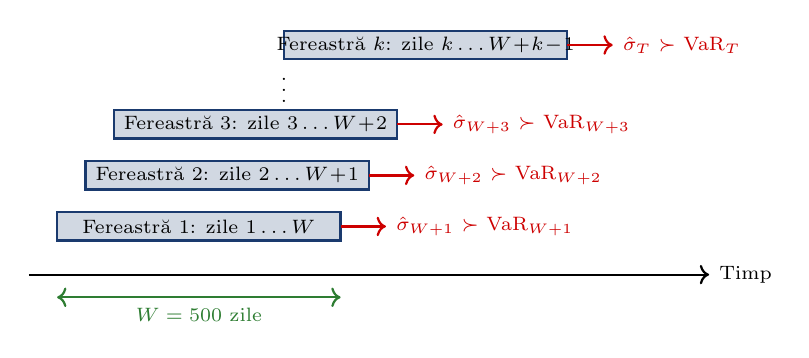
\begin{tikzpicture}[scale=0.72, every node/.style={font=\scriptsize}]
        % Timeline
        \draw[->, thick] (0,0) -- (12,0) node[right] {Timp};

        % Window 1
        \draw[fill=MainBlue!20, draw=MainBlue, thick] (0.5,0.6) rectangle (5.5,1.1);
        \node at (3,0.85) {Fereastră 1: zile $1 \ldots W$};
        \draw[->, thick, IDAred] (5.5,0.85) -- (6.3,0.85) node[right] {$\hat{\sigma}_{W+1}$ $\succ$ VaR$_{W+1}$};

        % Window 2
        \draw[fill=MainBlue!20, draw=MainBlue, thick] (1.0,1.5) rectangle (6.0,2.0);
        \node at (3.5,1.75) {Fereastră 2: zile $2 \ldots W\!+\!1$};
        \draw[->, thick, IDAred] (6.0,1.75) -- (6.8,1.75) node[right] {$\hat{\sigma}_{W+2}$ $\succ$ VaR$_{W+2}$};

        % Window 3
        \draw[fill=MainBlue!20, draw=MainBlue, thick] (1.5,2.4) rectangle (6.5,2.9);
        \node at (4,2.65) {Fereastră 3: zile $3 \ldots W\!+\!2$};
        \draw[->, thick, IDAred] (6.5,2.65) -- (7.3,2.65) node[right] {$\hat{\sigma}_{W+3}$ $\succ$ VaR$_{W+3}$};

        % Dots
        \node at (4.5,3.4) {$\vdots$};

        % Window T
        \draw[fill=MainBlue!20, draw=MainBlue, thick] (4.5,3.8) rectangle (9.5,4.3);
        \node at (7,4.05) {Fereastră $k$: zile $k \ldots W\!+\!k\!-\!1$};
        \draw[->, thick, IDAred] (9.5,4.05) -- (10.3,4.05) node[right] {$\hat{\sigma}_{T}$ $\succ$ VaR$_{T}$};

        % Annotations
        \draw[<->, thick, Forest] (0.5,-0.4) -- (5.5,-0.4) node[midway, below] {$W = 500$ zile};
    \end{tikzpicture}
    \end{center}
    \vspace{-0.2cm}
    {\small
    \begin{block}{Rezultat}
        \begin{itemize}\setlength{\itemsep}{0pt}
            \item Obținem seria $\{\text{VaR}_{\alpha,t}\}_{t=W+1}^{T}$ $\succ$ un prag \textbf{diferit} în fiecare zi
            \item VaR-ul se adaptează la regimul curent: crește în perioadele volatile, scade în cele calme
            \item Comparăm $r_t$ cu $-\text{VaR}_{\alpha,t}$ pentru a identifica încălcările
        \end{itemize}
    \end{block}
    }
    \end{cminipage}
\end{frame}

\begin{frame}{Prognoza volatilității cu intervale de încredere}
    \vspace{-0.2cm}
    {\scriptsize
    \begin{block}{Interpretare}
        \begin{itemize}\setlength{\itemsep}{0pt}
            \item Prognoza converge către $\bar{\sigma}$
            \item Incertitudinea crește cu orizontul de prognoză
        \end{itemize}
    \end{block}
    }
    \begin{center}
        \includegraphics[width=0.95\textwidth, height=0.50\textheight, keepaspectratio]{garch_volatility_forecast.pdf}
    \end{center}
    \quantlet{TSA\_ch5\_vol\_ci}{https://github.com/QuantLet/TSA/tree/main/TSA_ch5/TSA_ch5_vol_ci}
\end{frame}

\begin{frame}{Backtesting complet $\succ$ rezultate și decizie}
\small
\begin{block}{Aplicare S\&P 500 (T=500, VaR 1\%)}
\end{block}
\begin{exampleblock}{Output tipic}
\end{exampleblock}
    \quantlet{TSA\_ch5\_backtest\_full}{https://github.com/QuantLet/TSA/tree/main/TSA_ch5/TSA_ch5_backtest_full}
\end{frame}

\begin{frame}{Rolling forecast $\succ$ prognoza pas cu pas}
    \vspace{-0.2cm}
    {\scriptsize
    \begin{block}{Procedura}
        {\footnotesize
            S\&P 500, W=500, GARCH(1,1)-t
            \begin{itemize}\setlength{\itemsep}{1pt}
                \item Re-estimare GARCH pe $[t\!-\!W,\; t\!-\!1]$; prognoză $\hat{\sigma}_{t|t-1}$
                \item Comparație cu vol.\ realizată (std.\ rulantă 20 zile)
            \end{itemize}
        }
        \end{block}
        \vspace{-0.1cm}
        \begin{exampleblock}{Rezultate (2015 zile OOS)}
        {\footnotesize
            \begin{itemize}\setlength{\itemsep}{1pt}
                \item $\rho = 0.938$ $\succ$ urmărire excelentă; MAE $= 0.15\%$, RMSE $= 0.24\%$
                \item COVID-19: sub-predicție temporară, adaptare rapidă
            \end{itemize}
        }
        \end{exampleblock}
    }
    \begin{center}
        \includegraphics[width=0.95\textwidth, height=0.25\textheight, keepaspectratio]{garch_rolling_forecast.pdf}
    \end{center}
    \quantlet{TSA\_ch5\_rolling\_forecast}{https://github.com/QuantLet/TSA/tree/main/TSA_ch5/TSA_ch5_rolling_forecast}
\end{frame}

%=============================================================================
% SECȚIUNEA 7: IMPLEMENTARE ÎN PYTHON
%=============================================================================
%=============================================================================
% SECȚIUNEA 7b: MODELARE COMBINATĂ ARMA-GARCH
%=============================================================================

\begin{frame}{ARMA-GARCH: modelarea combinată a mediei și varianței}
\small
    \begin{cminipage}{0.95\textwidth}
    \begin{block}{De ce modelare combinată?}
        \begin{itemize}\setlength{\itemsep}{0pt}
            \item \textbf{Corelație serială} $\succ$ ARMA pentru medie
                \begin{itemize}\setlength{\itemsep}{0pt}
                    \item Captează dependența liniară în randamente
                \end{itemize}
            \item \textbf{Volatility clustering} $\succ$ GARCH pentru varianță
                \begin{itemize}\setlength{\itemsep}{0pt}
                    \item Captează dependența neliniară (heteroscedasticitate)
                \end{itemize}
        \end{itemize}
    \end{block}
    \vspace{-0.1cm}
    \begin{defn}[ARMA(p,q)-GARCH(r,s)]
        \begin{itemize}\setlength{\itemsep}{0pt}
            \item \textbf{Ecuația mediei}: $r_t = \mu + \sum_{i=1}^{p} \phi_i (r_{t-i} - \mu) + \sum_{j=1}^{q} \theta_j \varepsilon_{t-j} + \varepsilon_t$
            \item \textbf{Ecuația varianței}: $\varepsilon_t = \sigma_t z_t$, \quad $\sigma_t^2 = \omega + \sum_{i=1}^{r} \alpha_i \varepsilon_{t-i}^2 + \sum_{j=1}^{s} \beta_j \sigma_{t-j}^2$
        \end{itemize}
    \end{defn}
    \end{cminipage}
\end{frame}

\begin{frame}{ARMA-GARCH: strategie de selecție a modelului}
\small
    \begin{cminipage}{0.95\textwidth}
    \begin{block}{Abordare pas cu pas}
        \begin{enumerate}\setlength{\itemsep}{0pt}
            \item \textbf{Identifică modelul pentru medie}: Verifică ACF/PACF al randamentelor
            \item \textbf{Testează efectele ARCH}: Aplică testul ARCH-LM pe reziduuri
            \item \textbf{Specifică modelul pentru varianță}: De obicei GARCH(1,1) este suficient
            \item \textbf{Estimare combinată}: Estimează ambele ecuații prin MLE
            \item \textbf{Diagnostic}: Reziduurile standardizate trebuie să fie i.i.d.
        \end{enumerate}
    \end{block}
    \vspace{-0.2cm}
    \begin{alertblock}{Specificații comune}
        \begin{itemize}\setlength{\itemsep}{0pt}
            \item \textbf{Randamente acțiuni}: AR(1)-GARCH(1,1) sau ARMA(1,1)-GARCH(1,1)
                \begin{itemize}\setlength{\itemsep}{0pt}
                    \item Leverage effect frecvent $\succ$ EGARCH poate fi preferat
                \end{itemize}
            \item \textbf{Cursuri de schimb}: Adesea doar GARCH(1,1)
                \begin{itemize}\setlength{\itemsep}{0pt}
                    \item Fără dinamică semnificativă în medie
                \end{itemize}
            \item \textbf{Rate ale dobânzii}: AR(1)-EGARCH(1,1) pentru efecte de levier
        \end{itemize}
    \end{alertblock}
    \end{cminipage}
\end{frame}

%=============================================================================
% SECȚIUNEA 8: STUDIU DE CAZ --- S&P 500
%=============================================================================
\section{Studiu de Caz: S\&P 500}

\begin{frame}{Pasul 1: Datele $\succ$ randamente zilnice S\&P 500}
    \vspace{-0.2cm}
    {\scriptsize
    {\small
        \begin{block}{Descrierea datelor}
            \begin{itemize}\setlength{\itemsep}{0pt}
                \item \textbf{Sursă}: Yahoo Finance, S\&P 500, date zilnice 2000--2024 ($T > 6000$)
                \item \textbf{Randamente}: $r_t = \ln(P_t/P_{t-1}) \times 100$
            \end{itemize}
        \end{block}
        \vspace{-0.2cm}
        \begin{exampleblock}{Statistici descriptive}
            \vspace{-0.1cm}
            \begin{center}
            {\footnotesize
            \begin{tabular}{cccccc}
                \toprule
                Medie & Std. Dev. & Skewness & Kurtosis & Min & Max \\
                \midrule
                0.034\% & 1.21\% & $-0.29$ & 13.8 & $-12.8\%$ & $+11.0\%$ \\
                \bottomrule
            \end{tabular}
            }
            \end{center}
            \vspace{-0.1cm}
            \begin{itemize}\setlength{\itemsep}{0pt}
                \item Cozi groase (kurtosis $\gg 3$) și asimetrie negativă $\succ$ efecte ARCH
            \end{itemize}
        \end{exampleblock}
        }
    }
    \begin{center}
        \includegraphics[width=0.95\textwidth, height=0.23\textheight, keepaspectratio]{garch_sp500_returns.pdf}
    \end{center}
    \quantlet{TSA\_ch5\_sp500}{https://github.com/QuantLet/TSA/tree/main/TSA_ch5/TSA_ch5_sp500}
\end{frame}

\begin{frame}{Pasul 2: Testarea efectelor ARCH}
    \small
    \begin{block}{Cod Python $\succ$ ARCH-LM și Ljung-Box pe $r_t^2$}
    \end{block}
    \begin{exampleblock}{Rezultate}
        {\small
        \begin{tabular}{lcc}
            \toprule
            \textbf{Test} & \textbf{Statistică} & \textbf{p-value} \\
            \midrule
            ARCH-LM (10 lags) & 892.4 & $< 0.0001$ \\
            Ljung-Box $r_t^2$ (lag 20) & 4217.6 & $< 0.0001$ \\
            \bottomrule
        \end{tabular}
        }
        \begin{itemize}\setlength{\itemsep}{0pt}
            \item \textbf{Concluzie}: Efecte ARCH puternice $\succ$ heteroscedasticitate semnificativă
        \end{itemize}
    \end{exampleblock}
\end{frame}

\begin{frame}{Pasul 3: Parametri estimați $\succ$ comparație}
    \vspace{-0.2cm}
    {\scriptsize
    {\scriptsize
        \begin{block}{Tabel parametri estimați}
            \begin{center}
            \begin{tabular}{lccccccc}
                \toprule
                \textbf{Model} & $\omega$ & $\alpha$ & $\beta$ & $\gamma$ & $\alpha\!+\!\beta$ & $\nu$ & \textbf{HL} \\
                \midrule
                GARCH-N & 0.011 & 0.088 & 0.901 & --- & 0.989 & --- & 60 zile \\
                GARCH-t & 0.011 & 0.088 & 0.900 & --- & 0.989 & 6.42 & 60 zile \\
                EGARCH-t & 0.003 & 0.103 & 0.987 & $-$0.120 & --- & 6.38 & --- \\
                GJR-t & 0.010 & 0.022 & 0.906 & 0.126 & 0.991 & 6.51 & 78 zile \\
                \bottomrule
            \end{tabular}
            \end{center}
        \end{block}
        \vspace{-0.1cm}
        \begin{alertblock}{Interpretare}
            \begin{itemize}\setlength{\itemsep}{0pt}
                \item EGARCH $\gamma = -0.12$ \textbf{semnificativ} $\succ$ \textbf{leverage effect confirmat}
                \item GJR: $\alpha_{\text{neg}} = \alpha + \gamma = 0.148$ vs $\alpha_{\text{poz}} = 0.022$ $\succ$ asimetrie puternică
            \end{itemize}
        \end{alertblock}
        }
    }
    \begin{center}
        \includegraphics[width=0.95\textwidth, height=0.18\textheight, keepaspectratio]{garch_sp500_volatility.pdf}
    \end{center}
    \quantlet{TSA\_ch5\_sp500\_garch}{https://github.com/QuantLet/TSA/tree/main/TSA_ch5/TSA_ch5_sp500_garch}
\end{frame}

\begin{frame}{Pasul 5: Diagnostice $\succ$ EGARCH(1,1)-t}
    \vspace{-0.2cm}
    {\footnotesize
    \begin{block}{Verificări pe reziduuri standardizate $z_t = \varepsilon_t / \hat{\sigma}_t$}
            \begin{itemize}\setlength{\itemsep}{0pt}
                \item \textbf{Ljung-Box} pe $z_t$: p-value $= 0.38$ $\succ$ fără autocorelație reziduală
                \item \textbf{Ljung-Box} pe $z_t^2$: p-value $= 0.52$ $\succ$ \textbf{efecte ARCH eliminate}
                \item \textbf{Q-Q plot}: punctele urmează dreapta teoretică Student-t
                \item \textbf{Concluzie}: modelul EGARCH(1,1)-t captează adecvat dinamica volatilității
            \end{itemize}
        \end{block}
    }
    \begin{center}
        \includegraphics[width=0.95\textwidth, height=0.47\textheight, keepaspectratio]{garch_diagnostics.pdf}
    \end{center}
    \quantlet{TSA\_ch5\_sp500\_diag}{https://github.com/QuantLet/TSA/tree/main/TSA_ch5/TSA_ch5_sp500_diag}
\end{frame}

\begin{frame}{Pasul 4: Selecția modelului $\succ$ AIC/BIC}
    \begin{cminipage}{0.95\textwidth}
    \begin{block}{Criterii informaționale}
        \begin{center}
        {\small
        \begin{tabular}{lcccl}
            \toprule
            \textbf{Model} & \textbf{Log-Lik} & \textbf{AIC} & \textbf{BIC} & \textbf{Rang} \\
            \midrule
            GARCH(1,1)-N & $-$8042.3 & 16090.6 & 16111.0 & 4 \\
            GARCH(1,1)-t & $-$7981.5 & 15971.0 & 15997.8 & 3 \\
            EGARCH(1,1)-t & $-$7964.2 & \textbf{15938.4} & \textbf{15971.6} & \textbf{1} \\
            GJR-GARCH(1,1)-t & $-$7968.1 & 15946.2 & 15979.4 & 2 \\
            \bottomrule
        \end{tabular}
        }
        \end{center}
    \end{block}
    \begin{exampleblock}{Decizia}
        \begin{itemize}\setlength{\itemsep}{0pt}
            \item \textbf{EGARCH(1,1)-t câștigă}: cel mai mic AIC \textbf{și} BIC
            \item Student-t superior normalei ($\Delta$AIC $\approx 120$) $\succ$ cozi groase contează!
            \item Leverage effect justifică modele asimetrice ($\Delta$AIC $\approx 33$ față de GARCH-t)
        \end{itemize}
    \end{exampleblock}
    \end{cminipage}
\end{frame}

\begin{frame}{Pasul 5: Leverage effect $\succ$ vizualizare}
    \vspace{-0.2cm}
    {\footnotesize
    \begin{block}{GARCH vs EGARCH $\succ$ diferențe de volatilitate}
            \begin{itemize}\setlength{\itemsep}{0pt}
                \item EGARCH produce volatilitate \textbf{mai mare} după șocuri negative (2008, 2020)
                \item GARCH simetric \textbf{subestimează} riscul în perioadele de criză
                \item Diferența: până la 2--3 puncte procentuale în volatilitate zilnică
            \end{itemize}
        \end{block}
    }
    \begin{center}
        \includegraphics[width=0.95\textwidth, height=0.50\textheight, keepaspectratio]{garch_sp500_comparison.pdf}
    \end{center}
    \quantlet{TSA\_ch5\_sp500\_comp}{https://github.com/QuantLet/TSA/tree/main/TSA_ch5/TSA_ch5_sp500_comp}
\end{frame}

\begin{frame}{Pasul 6: Backtesting rolling VaR $\succ$ S\&P 500}
    \vspace{-0.2cm}
    {\scriptsize
    {\small
        \begin{exampleblock}{Rezultate Kupiec + Christoffersen (2015 zile out-of-sample)}
            \vspace{-0.1cm}
            \begin{center}
            {\footnotesize
            \begin{tabular}{lccl}
                \toprule
                \textbf{Test} & \textbf{Statistică} & \textbf{p-value} & \textbf{Decizia} \\
                \midrule
                Încălcări & 27/2015 ($\hat{p}=1.34\%$) & --- & Zona \textcolor{Forest}{\textbf{verde}} \\
                Kupiec (uc) & 2.13 & 0.145 & \textcolor{Forest}{Acceptat} \\
                Christoffersen (ind) & 0.79 & 0.375 & \textcolor{Forest}{Acceptat} \\
                Combinat (cc) & 2.91 & 0.233 & \textcolor{Forest}{Acceptat} \\
                \bottomrule
            \end{tabular}
            }
            \end{center}
        \end{exampleblock}
        }
    }
    \begin{center}
        \includegraphics[width=0.95\textwidth, height=0.41\textheight, keepaspectratio]{garch_sp500_rolling_var.pdf}
    \end{center}
    \quantlet{TSA\_ch5\_sp500\_var}{https://github.com/QuantLet/TSA/tree/main/TSA_ch5/TSA_ch5_sp500_var}
\end{frame}

\begin{frame}{Pasul 7: Concluzii $\succ$ studiu S\&P 500}
    \begin{cminipage}{0.95\textwidth}
    \begin{block}{Rezumatul metodologiei pas cu pas}
        \begin{enumerate}\setlength{\itemsep}{2pt}
            \item \textbf{Date}: randamente log, statistici descriptive $\succ$ cozi groase, asimetrie
            \item \textbf{Test ARCH}: ARCH-LM + Ljung-Box pe $r_t^2$ $\succ$ efecte ARCH semnificative
            \item \textbf{Estimare}: 4 modele candidate (simetric/asimetric $\times$ Normal/Student-t)
            \item \textbf{Selecție}: AIC/BIC $\succ$ \textbf{EGARCH(1,1)-t} câștigător
            \item \textbf{Diagnostice}: reziduuri standardizate $\succ$ model adecvat
            \item \textbf{VaR}: rolling window + backtesting Kupiec/Christoffersen $\succ$ model \textbf{validat}
        \end{enumerate}
    \end{block}
    \vspace{0.1cm}
    \begin{alertblock}{Lecții cheie}
        \begin{itemize}\setlength{\itemsep}{0pt}
            \item Distribuția Student-t este \textbf{esențială} pentru date financiare
            \item Leverage effect: modelele asimetrice \textbf{obligatorii} pentru acțiuni
            \item Backtesting sistematic: nu doar „arată bine'', ci \textbf{testat statistic}
        \end{itemize}
    \end{alertblock}
    \end{cminipage}
\end{frame}

%=============================================================================
% SECȚIUNEA 9: STUDIU DE CAZ --- Bitcoin
%=============================================================================
\section{Studiu de Caz: Bitcoin}

\begin{frame}{Pasul 1: Datele $\succ$ randamente zilnice Bitcoin}
    \vspace{-0.2cm}
    {\scriptsize
        \begin{block}{Descrierea datelor}
            \begin{itemize}\setlength{\itemsep}{0pt}
                \item \textbf{Sursă}: Yahoo Finance (BTC-USD), date zilnice 2018--2024
                \item Randamente log: media $\approx 0.05\%$, volatilitate $\approx 3.5\%$
            \end{itemize}
        \end{block}
        \vspace{-0.2cm}
        \begin{exampleblock}{Statistici descriptive}
            \vspace{-0.1cm}
            \begin{center}
            {\footnotesize
            \begin{tabular}{cccccc}
                \toprule
                Medie & Std. Dev. & Skewness & Kurtosis & Min & Max \\
                \midrule
                0.05\% & 3.48\% & $-0.72$ & 12.1 & $-46.5\%$ & $+22.5\%$ \\
                \bottomrule
            \end{tabular}
            }
            \end{center}
            \vspace{-0.15cm}
            \begin{itemize}\setlength{\itemsep}{0pt}
                \item Volatilitate $\sim$3$\times$ mai mare decât S\&P 500
                \item Kurtosis extremă $\succ$ riscul de pierderi mari
            \end{itemize}
        \end{exampleblock}
        }
    \begin{center}
        \includegraphics[width=0.95\textwidth, height=0.19\textheight, keepaspectratio]{btc_returns.pdf}
    \end{center}
    \quantlet{TSA\_ch5\_btc}{https://github.com/QuantLet/TSA/tree/main/TSA_ch5/TSA_ch5_btc}
\end{frame}

\begin{frame}{Pasul 2: Testarea efectelor ARCH $\succ$ Bitcoin}
    \vspace{-0.2cm}
    {\scriptsize
    }
    \begin{center}
        \includegraphics[width=0.95\textwidth, height=0.50\textheight, keepaspectratio]{btc_squared_returns.pdf}
    \end{center}
    \quantlet{TSA\_ch5\_btc\_arch}{https://github.com/QuantLet/TSA/tree/main/TSA_ch5/TSA_ch5_btc_arch}
\end{frame}

\begin{frame}{Pasul 5: Volatilitatea condiționată $\succ$ Bitcoin}
    \vspace{-0.2cm}
    {\footnotesize
    \begin{block}{Diagnostice GJR-GARCH(1,1)-t}
            \begin{itemize}\setlength{\itemsep}{0pt}
                \item Ljung-Box pe $z_t^2$: p-value $= 0.41$ $\succ$ \textbf{efecte ARCH eliminate}
                \item Vârfuri volatilitate: martie 2020 (COVID), mai 2022 (Terra/Luna)
                \item Volatilitate zilnică: de la 1\% (perioadele calme) la $>$15\% (crize)
            \end{itemize}
        \end{block}
    }
    \begin{center}
        \includegraphics[width=0.95\textwidth, height=0.50\textheight, keepaspectratio]{ch10_bitcoin_garch.pdf}
    \end{center}
    \quantlet{TSA\_ch5\_btc\_garch}{https://github.com/QuantLet/TSA/tree/main/TSA_ch5/TSA_ch5_btc_garch}
\end{frame}

\begin{frame}{Pasul 3--4: Estimare și selecție modele $\succ$ Bitcoin}
    \begin{cminipage}{0.95\textwidth}
    \begin{block}{Parametri estimați}
        \begin{center}
        {\small
        \begin{tabular}{lccccccc}
            \toprule
            \textbf{Model} & $\omega$ & $\alpha$ & $\beta$ & $\gamma$ & $\alpha\!+\!\beta$ & $\nu$ & \textbf{AIC} \\
            \midrule
            GARCH-t & 0.42 & 0.131 & 0.848 & --- & 0.979 & 4.82 & 9284 \\
            EGARCH-t & 0.08 & 0.184 & 0.976 & $-$0.061 & --- & 4.79 & 9276 \\
            GJR-t & 0.40 & 0.088 & 0.854 & 0.078 & 0.976 & 4.85 & \textbf{9271} \\
            \bottomrule
        \end{tabular}
        }
        \end{center}
    \end{block}
    \begin{block}{Interpretare}
        \begin{itemize}\setlength{\itemsep}{0pt}
            \item \textbf{GJR-GARCH-t câștigă} (cel mai mic AIC)
            \item $\nu \approx 4.8$: cozi \textbf{mult mai groase} decât S\&P 500 ($\nu = 6.4$)
            \item $\alpha = 0.131$ (BTC) vs $0.088$ (S\&P) $\succ$ Bitcoin reacționează mai rapid la news
            \item Leverage effect mai slab decât la acțiuni ($\gamma_{\text{BTC}} = 0.078$ vs $0.126$)
        \end{itemize}
    \end{block}
    \end{cminipage}
\end{frame}

\begin{frame}{Pasul 6: Backtesting rolling VaR $\succ$ Bitcoin}
    \vspace{-0.2cm}
    {\scriptsize
    {\scriptsize
        \begin{block}{Teste statistice (2421 zile out-of-sample)}
            \vspace{-0.15cm}
            \begin{center}
            \begin{tabular}{lccl}
                \toprule
                \textbf{Test} & \textbf{Statistică} & \textbf{p-value} & \textbf{Decizia} \\
                \midrule
                Încălcări & 28/2421 ($\hat{p}=1.16\%$) & --- & Zona \textcolor{Forest}{\textbf{verde}} \\
                Kupiec (uc) & 0.57 & 0.450 & \textcolor{Forest}{Acceptat} \\
                Christoffersen (ind) & 0.94 & 0.333 & \textcolor{Forest}{Acceptat} \\
                Combinat (cc) & 1.51 & 0.471 & \textcolor{Forest}{Acceptat} \\
                \bottomrule
            \end{tabular}
            \end{center}
            \vspace{-0.15cm}
        \end{block}
        \vspace{-0.15cm}
        \begin{alertblock}{Interpretare}
            \begin{itemize}\setlength{\itemsep}{0pt}
                \item Volatilitatea variază de la 3\% la 38\% $\succ$ rolling window \textbf{esențial}
                \item Toate testele \textbf{acceptate}: model valid pentru managementul riscului
            \end{itemize}
        \end{alertblock}
        }
    }
    \begin{center}
        \includegraphics[width=0.95\textwidth, height=0.22\textheight, keepaspectratio]{garch_btc_rolling_var.pdf}
    \end{center}
    \quantlet{TSA\_ch5\_btc\_var}{https://github.com/QuantLet/TSA/tree/main/TSA_ch5/TSA_ch5_btc_var}
\end{frame}

\begin{frame}{Pasul 6: VaR rolling window $\succ$ Bitcoin}
    \small
    \begin{block}{Rolling window GJR-GARCH-t (W=500 zile, VaR 1\%)}
    \end{block}
    {\small
    \begin{exampleblock}{Caracteristici VaR rolling Bitcoin (2018--2024)}
        \begin{itemize}\setlength{\itemsep}{0pt}
            \item VaR mediu: 9.34\% ($\approx$ EUR 93.400 / 1M EUR)
            \item VaR maxim: 37.54\% $\succ$ crash COVID martie 2020
            \item VaR minim: 2.90\% $\succ$ perioadă calmă
            \item Bitcoin: VaR rolling $\sim$4$\times$ mai mare decât S\&P 500 la aceeași expunere
        \end{itemize}
    \end{exampleblock}
    }
\end{frame}

\begin{frame}{Comparație finală: S\&P 500 vs Bitcoin}
    \vspace{-0.3cm}
    \begin{cminipage}{0.95\textwidth}
    {\small
    \begin{block}{Rezumat comparativ}
        \vspace{-0.1cm}
        \begin{center}
        {\footnotesize
        \begin{tabular}{lcc}
            \toprule
            & \textbf{S\&P 500} & \textbf{Bitcoin} \\
            \midrule
            Volatilitate medie & 1.2\% & 3.5\% \\
            Kurtosis & 13.8 & 12.1 \\
            Student-t $\nu$ & 6.42 & 4.82 \\
            Cel mai bun model & EGARCH(1,1)-t & GJR-GARCH(1,1)-t \\
            Leverage effect & Puternic ($\gamma = -0.12$) & Moderat ($\gamma = 0.078$) \\
            Half-life & $\sim$60 zile & $\sim$42 zile \\
            Rolling VaR 1\% mediu & 2.53\% & 9.34\% \\
            Rolling VaR 1\% maxim & 22.02\% (COVID) & 37.54\% (COVID) \\
            Kupiec & \textcolor{Forest}{\textbf{Acceptat}} (p=0.145) & \textcolor{Forest}{\textbf{Acceptat}} (p=0.450) \\
            Christoffersen (ind) & \textcolor{Forest}{\textbf{Acceptat}} (p=0.375) & \textcolor{Forest}{\textbf{Acceptat}} (p=0.333) \\
            \bottomrule
        \end{tabular}
        }
        \end{center}
    \end{block}
    \vspace{-0.1cm}
    \begin{alertblock}{Concluzie generală}
        \begin{itemize}\setlength{\itemsep}{0pt}
            \item Re-estimare GARCH la fiecare pas: Kupiec + Christoffersen \textbf{acceptate}
            \item Rolling window VaR: \textbf{obligatoriu} $\succ$ VaR static complet inadecvat
            \item Student-t + model asimetric: \textbf{esențiale} pentru ambele piețe
        \end{itemize}
    \end{alertblock}
    }
    \end{cminipage}
\end{frame}

%=============================================================================
% FORMULE CHEIE
%=============================================================================
\begin{frame}{Formule cheie}
\small
    \begin{cminipage}{0.95\textwidth}
    \begin{block}{Modele de volatilitate}
        \begin{itemize}\setlength{\itemsep}{0pt}
            \item \textbf{ARCH(q):} $\sigma_t^2 = \omega + \sum_{i=1}^{q} \alpha_i \varepsilon_{t-i}^2$
            \item \textbf{GARCH(1,1):} $\sigma_t^2 = \omega + \alpha \varepsilon_{t-1}^2 + \beta \sigma_{t-1}^2$
            \item \textbf{EGARCH:} $\ln(\sigma_t^2) = \omega + \alpha(|z_{t-1}| - \E[|z|]) + \gamma z_{t-1} + \beta \ln(\sigma_{t-1}^2)$
            \item \textbf{GJR-GARCH:} $\sigma_t^2 = \omega + \alpha \varepsilon_{t-1}^2 + \gamma \varepsilon_{t-1}^2 I_{t-1} + \beta \sigma_{t-1}^2$
        \end{itemize}
    \end{block}
    \vspace{-0.1cm}
    \begin{block}{Proprietăți și măsuri}
        \begin{itemize}\setlength{\itemsep}{0pt}
            \item \textbf{Var. necond.:} $\bar{\sigma}^2 = \frac{\omega}{1-\alpha-\beta}$ \quad $\mid$ \quad \textbf{Half-life:} $HL = \frac{\ln(0.5)}{\ln(\alpha+\beta)}$ \quad $\mid$ \quad \textbf{VaR:} $\text{VaR}_\alpha = z_\alpha \cdot \sigma_{T+1}$
        \end{itemize}
    \end{block}
    \vspace{-0.1cm}
    \begin{alertblock}{Test ARCH-LM}
        \begin{itemize}\setlength{\itemsep}{0pt}
            \item \textbf{Statistica}: $LM = T \cdot R^2 \sim \chi^2(q)$ unde $R^2$ provine din regresia $\hat{\varepsilon}_t^2$ pe lag-urile sale
            \item \textbf{Staționaritate}: $\alpha + \beta < 1$
        \end{itemize}
    \end{alertblock}
    \end{cminipage}
\end{frame}

%=============================================================================
\section{Utilizare IA}
%=============================================================================

\begin{frame}{Exercițiu AI: Gândire critică}
    \vspace{-3mm}
    \begin{cminipage}{0.95\textwidth}
    \begin{block}{\footnotesize Prompt de testat în ChatGPT / Claude / Copilot}
        {\footnotesize
        ``Folosind yfinance, descarcă prețurile zilnice de închidere S\&P 500 (\^{}GSPC) din 2018-01-01 până în 2024-12-31 (aprox.\ 1.750 observații). Calculează randamentele logaritmice zilnice. Testează efectele ARCH, ajustează un model GARCH(1,1) și prognozează volatilitatea pe următoarele 20 de zile de tranzacționare. Vreau cod Python complet.''
        }
    \end{block}
    \vspace{-2mm}
    {\footnotesize
    \textbf{Exercițiu}:
    \begin{enumerate}\setlength{\itemsep}{0pt}
        \item Rulați prompt-ul într-un LLM la alegere și analizați critic răspunsul.
        \item Calculează randamentele logaritmice corect? Elimină media înainte de GARCH?
        \item Cum testează efectele ARCH? Folosește testul LM al lui Engle?
        \item Separă ecuația mediei de ecuația varianței?
        \item Discută efectele asimetrice (GJR-GARCH, EGARCH)? Estimările VaR sunt calculate din distribuția condițională?
    \end{enumerate}
    }
    \vspace{-2mm}
    \begin{alertblock}{}
        {\footnotesize \textbf{Atenție}: Codul generat de AI poate rula fără erori și arăta profesional. \textit{Asta nu înseamnă că e corect.}}
    \end{alertblock}
    \end{cminipage}
\end{frame}

%=============================================================================
% REZUMAT
%=============================================================================
\section{Rezumat}

\begin{frame}{Rezumat $\succ$ capitolul 5: Modele de volatilitate}
\small
    \vspace{-0.2cm}
    \begin{cminipage}{0.95\textwidth}
    \begin{block}{Concepte cheie}
        \begin{itemize}\setlength{\itemsep}{0pt}
            \item \textbf{ARCH(q)}: varianța condiționată depinde de pătratele erorilor trecute (Nobel 2003)
            \item \textbf{GARCH(p,q)}: adaugă lag-uri ale varianței pentru persistență (GARCH(1,1) în 90\% din cazuri)
            \item \textbf{EGARCH}: permite leverage effect, fără restricții de pozitivitate
            \item \textbf{GJR-GARCH/TGARCH}: captură asimetria cu variabile indicador
        \end{itemize}
    \end{block}
    \vspace{-0.2cm}
    \begin{block}{Aplicații}
        \begin{itemize}\setlength{\itemsep}{0pt}
            \item Măsurarea și prognoza riscului (VaR, ES)
            \item Prețul derivatelor, hedging dinamic, managementul portofoliului
        \end{itemize}
    \end{block}
    \vspace{-0.2cm}
    \begin{alertblock}{Sfat practic}
        \begin{itemize}\setlength{\itemsep}{0pt}
            \item Începe cu GARCH(1,1), verifică leverage effect, alege distribuția care minimizează AIC/BIC!
                \begin{itemize}\setlength{\itemsep}{0pt}
                    \item Student-t adesea superior distribuției normale
                \end{itemize}
        \end{itemize}
    \end{alertblock}
    \end{cminipage}
\end{frame}

%=============================================================================
% QUIZ
%=============================================================================
\section{Quiz}

\begin{frame}{Întrebarea 1}
    \begin{cminipage}{0.95\textwidth}
    \begin{alertblock}{Întrebare}
        \begin{itemize}\setlength{\itemsep}{0pt}
            \item Ce descrie cel mai bine fenomenul de \textit{volatility clustering} în seriile financiare?
        \end{itemize}
    \end{alertblock}

    \vspace{0.3cm}

    \begin{block}{Variante de răspuns}

        \textcolor{MainBlue}{\textbf{(A)}} Randamentele financiare sunt distribuite normal și independente\\[3pt]

        \textcolor{MainBlue}{\textbf{(B)}} Perioadele de volatilitate ridicată sunt urmate de perioade de volatilitate ridicată, și invers\\[3pt]

        \textcolor{MainBlue}{\textbf{(C)}} Volatilitatea este constantă în timp (homoscedasticitate)\\[3pt]

        \textcolor{MainBlue}{\textbf{(D)}} Corelația dintre randamente este întotdeauna pozitivă

    \end{block}
    \end{cminipage}
\end{frame}

\begin{frame}{Întrebarea 1: Răspuns}
    \begin{cminipage}{0.95\textwidth}
    \vspace{-0.2cm}
    \begin{center}
        \includegraphics[width=0.98\textwidth, height=0.58\textheight, keepaspectratio]{garch_quiz1_volatility_clustering.pdf}
    \end{center}
    \vspace{-3mm}
    {\small
    \begin{exampleblock}{Răspuns: (B)}
    \begin{itemize}\setlength{\itemsep}{0pt}
        \item Volatility clustering este un fapt stilizat fundamental. Implică faptul că varianța condiționată este \textbf{predictibilă}, motivând modelele ARCH/GARCH.
    \end{itemize}
    \end{exampleblock}
    }
    \hfill\quantlet{TSA\_ch5\_quiz1\_volatility\_clustering}{https://github.com/QuantLet/TSA/tree/main/TSA_ch5/TSA_ch5_quiz1_volatility_clustering}
    \end{cminipage}
\end{frame}

\begin{frame}{Întrebarea 2}
    \begin{cminipage}{0.95\textwidth}
    \begin{alertblock}{Întrebare}
        \begin{itemize}\setlength{\itemsep}{0pt}
            \item Care este diferența principală dintre un model ARCH(q) și un model GARCH(p,q)?
        \end{itemize}
    \end{alertblock}

    \vspace{0.3cm}

    \begin{block}{Variante de răspuns}

        \textcolor{MainBlue}{\textbf{(A)}} GARCH modelează media condiționată, ARCH modelează varianța\\[3pt]

        \textcolor{MainBlue}{\textbf{(B)}} ARCH include lag-uri ale varianței condiționate, GARCH nu\\[3pt]

        \textcolor{MainBlue}{\textbf{(C)}} GARCH adaugă lag-uri ale varianței condiționate ($\sigma_{t-j}^2$) pe lângă pătratele erorilor\\[3pt]

        \textcolor{MainBlue}{\textbf{(D)}} ARCH este mai parsimonios decât GARCH

    \end{block}
    \end{cminipage}
\end{frame}

\begin{frame}{Întrebarea 2: Răspuns}
    \begin{cminipage}{0.95\textwidth}
    \vspace{-0.2cm}
    \begin{center}
        \includegraphics[width=0.98\textwidth, height=0.58\textheight, keepaspectratio]{garch_quiz2_arch_vs_garch.pdf}
    \end{center}
    \vspace{-3mm}
    {\small
    \begin{exampleblock}{Răspuns: (C)}
    \begin{itemize}\setlength{\itemsep}{0pt}
        \item GARCH(1,1) captează aceeași persistență ca ARCH(q) cu doar 2 parametri în loc de $q$. În practică, GARCH(1,1) este suficient în 90\% din cazuri.
    \end{itemize}
    \end{exampleblock}
    }
    \hfill\quantlet{TSA\_ch5\_quiz2\_arch\_vs\_garch}{https://github.com/QuantLet/TSA/tree/main/TSA_ch5/TSA_ch5_quiz2_arch_vs_garch}
    \end{cminipage}
\end{frame}

\begin{frame}{Întrebarea 3}
    \begin{cminipage}{0.95\textwidth}
    \begin{alertblock}{Întrebare}
        \begin{itemize}\setlength{\itemsep}{0pt}
            \item Ce este \textit{leverage effect} și ce modele GARCH îl captează?
        \end{itemize}
    \end{alertblock}

    \vspace{0.3cm}

    \begin{block}{Variante de răspuns}

        \textcolor{MainBlue}{\textbf{(A)}} Șocurile pozitive cresc volatilitatea mai mult; captat de GARCH standard\\[3pt]

        \textcolor{MainBlue}{\textbf{(B)}} Șocurile negative cresc volatilitatea mai mult; captat de EGARCH și GJR-GARCH\\[3pt]

        \textcolor{MainBlue}{\textbf{(C)}} Volatilitatea este simetrică; captat de toate modelele GARCH\\[3pt]

        \textcolor{MainBlue}{\textbf{(D)}} Efectul de levier financiar asupra prețului acțiunilor; captat de IGARCH

    \end{block}
    \end{cminipage}
\end{frame}

\begin{frame}{Întrebarea 3: Răspuns}
    \begin{cminipage}{0.95\textwidth}
    \vspace{-0.2cm}
    \begin{center}
        \includegraphics[width=0.98\textwidth, height=0.58\textheight, keepaspectratio]{garch_quiz3_leverage_effect.pdf}
    \end{center}
    \vspace{-3mm}
    {\small
    \begin{exampleblock}{Răspuns: (B)}
    \begin{itemize}\setlength{\itemsep}{0pt}
        \item Scăderile de preț cresc volatilitatea \textbf{mai mult} decât creșterile de aceeași magnitudine. GARCH standard folosește $\varepsilon_{t-1}^2$, pierzând informația de semn.
    \end{itemize}
    \end{exampleblock}
    }
    \hfill\quantlet{TSA\_ch5\_quiz3\_leverage\_effect}{https://github.com/QuantLet/TSA/tree/main/TSA_ch5/TSA_ch5_quiz3_leverage_effect}
    \end{cminipage}
\end{frame}

\begin{frame}{Întrebarea 4}
    \begin{cminipage}{0.95\textwidth}
    \begin{alertblock}{Întrebare}
        \begin{itemize}\setlength{\itemsep}{0pt}
            \item Care este condiția de staționaritate pentru un model GARCH(1,1)?
        \end{itemize}
    \end{alertblock}

    \vspace{0.3cm}

    \begin{block}{Variante de răspuns}

        \textcolor{MainBlue}{\textbf{(A)}} $\alpha + \beta = 1$\\[3pt]

        \textcolor{MainBlue}{\textbf{(B)}} $\alpha > 0$ și $\beta > 0$\\[3pt]

        \textcolor{MainBlue}{\textbf{(C)}} $\alpha + \beta < 1$, cu $\omega > 0$, $\alpha \geq 0$, $\beta \geq 0$\\[3pt]

        \textcolor{MainBlue}{\textbf{(D)}} $\alpha \cdot \beta < 1$

    \end{block}
    \end{cminipage}
\end{frame}

\begin{frame}{Întrebarea 4: Răspuns}
    \begin{cminipage}{0.95\textwidth}
    \vspace{-0.2cm}
    \begin{center}
        \includegraphics[width=0.98\textwidth, height=0.58\textheight, keepaspectratio]{garch_quiz4_stationarity.pdf}
    \end{center}
    \vspace{-3mm}
    {\small
    \begin{exampleblock}{Răspuns: (C)}
    \begin{itemize}\setlength{\itemsep}{0pt}
        \item Asigură existența varianței necondiționate finite: $\bar{\sigma}^2 = \frac{\omega}{1-\alpha-\beta}$. Când $\alpha + \beta = 1$ (IGARCH), varianța este infinită.
    \end{itemize}
    \end{exampleblock}
    }
    \hfill\quantlet{TSA\_ch5\_quiz4\_stationarity}{https://github.com/QuantLet/TSA/tree/main/TSA_ch5/TSA_ch5_quiz4_stationarity}
    \end{cminipage}
\end{frame}

\begin{frame}{Întrebarea 5}
    \begin{cminipage}{0.95\textwidth}
    \begin{alertblock}{Întrebare}
        \begin{itemize}\setlength{\itemsep}{0pt}
            \item Ce reprezintă \textit{half-life} al volatilității într-un model GARCH(1,1)?
        \end{itemize}
    \end{alertblock}

    \vspace{0.3cm}

    \begin{block}{Variante de răspuns}

        \textcolor{MainBlue}{\textbf{(A)}} Timpul necesar ca prețul să revină la media sa\\[3pt]

        \textcolor{MainBlue}{\textbf{(B)}} Numărul de perioade până când volatilitatea devine zero\\[3pt]

        \textcolor{MainBlue}{\textbf{(C)}} Numărul de perioade necesare ca un șoc de volatilitate să se reducă la jumătate\\[3pt]

        \textcolor{MainBlue}{\textbf{(D)}} Durata medie a unui episod de volatilitate ridicată

    \end{block}
    \end{cminipage}
\end{frame}

\begin{frame}{Întrebarea 5: Răspuns}
    \begin{cminipage}{0.95\textwidth}
    \vspace{-0.2cm}
    \begin{center}
        \includegraphics[width=0.98\textwidth, height=0.58\textheight, keepaspectratio]{garch_quiz5_halflife.pdf}
    \end{center}
    \vspace{-3mm}
    {\small
    \begin{exampleblock}{Răspuns: (C)}
    \begin{itemize}\setlength{\itemsep}{0pt}
        \item $HL = \frac{\ln(0.5)}{\ln(\alpha+\beta)}$. Exemplu: S\&P 500 cu $\alpha+\beta=0.988$ dă $HL \approx 58$ zile (șocurile persistă $\sim$3 luni).
    \end{itemize}
    \end{exampleblock}
    }
    \hfill\quantlet{TSA\_ch5\_quiz5\_halflife}{https://github.com/QuantLet/TSA/tree/main/TSA_ch5/TSA_ch5_quiz5_halflife}
    \end{cminipage}
\end{frame}

%=============================================================================
% BIBLIOGRAFIE
%=============================================================================
\begin{frame}{Bibliografie I}
    \begin{block}{Lucrări fundamentale ARCH/GARCH}
        {\small
        \begin{itemize}\setlength{\itemsep}{0pt}
            \item Engle, R.F. (1982). Autoregressive Conditional Heteroscedasticity with Estimates of the Variance of UK Inflation, \textit{Econometrica}, 50(4), 987--1007.
            \item Bollerslev, T. (1986). Generalized Autoregressive Conditional Heteroskedasticity, \textit{Journal of Econometrics}, 31(3), 307--327.
            \item Nelson, D.B. (1991). Conditional Heteroskedasticity in Asset Returns: A New Approach, \textit{Econometrica}, 59(2), 347--370.
        \end{itemize}
        }
    \end{block}

    \begin{exampleblock}{Modele asimetrice și extensii}
        {\small
        \begin{itemize}\setlength{\itemsep}{0pt}
            \item Glosten, L.R., Jagannathan, R., \& Runkle, D.E. (1993). On the Relation Between the Expected Value and the Volatility of the Nominal Excess Return on Stocks, \textit{Journal of Finance}, 48(5), 1779--1801.
            \item Francq, C., \& Zakoïan, J.-M. (2019). \textit{GARCH Models: Structure, Statistical Inference and Financial Applications}, 2nd ed., Wiley.
        \end{itemize}
        }
    \end{exampleblock}
\end{frame}

\begin{frame}{Bibliografie II}
    \begin{block}{Manuale și aplicații financiare}
        {\small
        \begin{itemize}\setlength{\itemsep}{0pt}
            \item Tsay, R.S. (2010). \textit{Analysis of Financial Time Series}, 3rd ed., Wiley.
            \item Franke, J., Härdle, W.K., \& Hafner, C.M. (2019). \textit{Statistics of Financial Markets}, 4th ed., Springer.
            \item McNeil, A.J., Frey, R., \& Embrechts, P. (2015). \textit{Quantitative Risk Management}, 2nd ed., Princeton University Press.
        \end{itemize}
        }
    \end{block}

    \begin{exampleblock}{Resurse online și cod}
        {\small
        \begin{itemize}\setlength{\itemsep}{0pt}
            \item \textbf{Quantlet}: \url{https://quantlet.com} $\succ$ Depozit de cod pentru statistică
            \item \textbf{Quantinar}: \url{https://quantinar.com} $\succ$ Platformă de învățare metode cantitative
            \item \textbf{GitHub TSA}: \url{https://github.com/QuantLet/TSA/tree/main/TSA_ch5} $\succ$ Cod Python pentru acest capitol
        \end{itemize}
        }
    \end{exampleblock}
\end{frame}

\begin{frame}{}
    \centering
    \Huge\textcolor{MainBlue}{Vă Mulțumim!}

    \vspace{1cm}

    \Large Întrebări?

    \vspace{0.8cm}

    \normalsize

    Materialele cursului sunt disponibile la: \url{https://danpele.github.io/Time-Series-Analysis/}

    \vspace{0.2cm}

    \href{https://quantlet.com}{\raisebox{-0.15em}{\includegraphics[height=0.8em]{ql_logo.png}} Quantlet} \hspace{0.5cm}
    \href{https://quantinar.com}{\raisebox{-0.15em}{\includegraphics[height=0.8em]{qr_logo.png}} Quantinar}
\end{frame}

\end{document}
